\documentclass{izumdbf}
\usepackage{etex}
\usepackage[lined,algonl,boxed,commentsnumbered]{algorithm2e}
\usepackage[usenames]{color}
\usepackage{amsmath}
\usepackage{amssymb} 
\usepackage{graphicx,color,psfrag}
\usepackage{enumerate}
\usepackage{rotating}
\usepackage{cite}
\usepackage{psfrag}
\usepackage{pstricks, pst-plot, pst-grad, pstricks-add}
\usepackage{tikz}
\usepackage{pgfplots}
\usepackage{url}
\usepackage{faktor}
\usepackage{lscape}
\usepackage{xcolor}
\usepackage{tabularx}
\usepackage{multirow}
%\usepackage{ctable}
\usepackage{float}
\usepackage{afterpage}
\usepackage{lineno} 
\usepackage{subfigure}
\usepackage{epstopdf}
\usepackage[utf8x]{inputenc} 
\usepackage{algorithmic}
\usepackage{setspace}
\usepackage{longtable}
\usetikzlibrary{positioning,shapes,shadows,arrows}
\usepackage{calrsfs}  
\DeclareMathAlphabet{\pazocal}{OMS}{zplm}{m}{n} 
\newcommand{\La}{\mathcal{L}}
\newcommand{\Lb}{\pazocal{L}}
\usepackage{array}
\usepackage{tablefootnote} 
\usepackage{caption} 
\usepackage{amsmath} 
\usepackage{listings}
\usepackage{color}
\usepackage{fancyhdr}

\numberwithin{algocf}{section}



\ToCLineisDotted 
\ToCChapterBold  

\setlength{\fboxsep}{0pt}

\newcommand{\plotPGFfile}{true} % PGF olarak DATA dosyaları çizilsin mi çizilmesin mi? Çizilmez ise dosyadan sadece data okunan kısım atlanıyor, resmin çerçevesi oluşturuluyor...
\definecolor{dkgreen}{rgb}{0,0.6,0}
\definecolor{gray}{rgb}{0.5,0.5,0.5}
\definecolor{mauve}{rgb}{0.58,0,0.82}

\lstset{frame=tb,
	language=Java, %Uygulamanın yazıldığı programlama dili, (Örnek kullanım chapter4.tex'te verilmiştir.)
	aboveskip=3mm,
	belowskip=3mm,
	showstringspaces=false,
	columns=flexible,
	basicstyle={\small\ttfamily},
	numbers=none,
	numberstyle=\tiny\color{gray},
	keywordstyle=\color{blue},
	commentstyle=\color{dkgreen},
	stringstyle=\color{mauve},
	breaklines=true,
	breakatwhitespace=true,
	tabsize=3
}


\author{Halil}{Sarıkaya}{031021037}{031021037@std.izu.edu.tr}{Elektrik-Elektronik Mühendisliği}%1. Öğrenci ad soyad mail adresi bolum
%\authorIki{Ad}{Soyad}{ogrenciNo}{ad.soyad@std.edu.tr}{bolum}%2. Öğrenci ad soyad mail adresi bolum

%%%%
%\authorUc{Ad}{Soyad}{ogrenciNo}{ad.soyad@std.izu.edu.tr}{bolum}%3 Öğrenci ad soyad mail adresi bolum
%\authorDort{Ad}{Soyad}{ogrenciNo}{ad.soyad@std.izu.edu.tr}{bolum}%4. Öğrenci ad soyad mail adresi bolum
%\authorBes{Ad}{Soyad}{ogrenciNo}{ad.soyad@std.izu.edu.tr}{bolum}%4. Öğrenci ad soyad mail adresi bolum
\anabilimdali{Elektrik-Elektronik Mühendisliği}
\anabilimdaliUpper{ELEKTRİK-ELEKTRONİK MÜHENDİSLİĞİ}

\date{7 Haziran 2026}
\Yil{2025-2026}
\Donem{Güz}
\teziyoneten{Mohammed JOUDA, Dr. Öğr. Üyesi} % Danisman
\raporNo{Final}

\kisaltmalar{6DOF & 6 Serbestlik Derecesi \\
AHRS & Ataletsel Yönelim ve Referans Sistemi \\
CPU & Merkezi İşlem Birimi \\
DMA & Doğrudan Bellek Erişimi \\
DRDY & Veri Hazır Sinyali \\
EKF & Genişletilmiş Kalman Filtresi \\
EXTI & Dış Kesme Denetleyicisi \\
FPU & Kayan Nokta İşlem Birimi \\
FSM & Uçuş Durum Makinesi / Sonlu Durum Makinesi \\
GNSS & Küresel Konumlama Sistemi \\
GPIO & Genel Amaçlı Giriş/Çıkış \\
GPS & Küresel Konumlama Sistemi \\
GUI & Grafiksel Kullanıcı Arayüzü \\
HAL & Donanım Soyutlama Katmanı \\
I2C & Tümleşik Devreler Arası Haberleşme \\
IMU & Ataletsel Ölçüm Birimi \\
ISR & Kesme Servis Rutini \\
IWDG & Bağımsız Bekçi Zamanlayıcısı \\
LoRa & Uzun Menzilli Radyo Teknolojisi \\
LSI & Dahili Düşük Hızlı Saat Osilatörü \\
NVIC & İç İçe Kesme Denetleyicisi \\
PIL & Döngüde İşlemci Testi \\
RAM & Rastgele Erişimli Bellek \\
RTOS & Gerçek Zamanlı İşletim Sistemi \\
RX & Veri Alma / Alıcı Hattı \\
SIT & Sensör İzleme Testi \\
SPI & Seri Çevresel Arayüz \\
SRAM & Statik Rastgele Erişimli Bellek \\
SUT & Sentetik Uçuş Testi \\
TX & Veri Gönderme / Verici Hattı \\
UART & Evrensel Eşzamansız Alıcı-Verici \\
USART & Evrensel Eşzamanlı/Eşzamansız Alıcı-Verici}
\sembollistesi{$\theta$ & Yönelim / Eğim açısı \\
$\alpha$ & Tamamlayıcı filtre katsayısı \\
$\omega$ & Açısal hız \\
$\Delta t$ & Örnekleme periyodu / Zaman adımı \\
$\mathbf{e}$ & Hata vektörü \\
$\hat{\mathbf{g}}$ & Tahmini yerçekimi yönelim vektörü \\
$\mathbf{a}_{norm}$ & Normalize edilmiş ivme vektörü \\
$q$ & Yönelim kuaterniyonu / Kalman süreç gürültüsü katsayısı \\
$\dot{q}$ & Kuaterniyon türevi \\
$\otimes$ & Kuaterniyon çarpımı operatörü \\
$\omega_{gyro}$ & Jiroskop ölçüm vektörü \\
$\mathbf{b}$ & Jiroskop sapma (bias) vektörü \\
$K_p$ & Mahony filtresi oransal kazancı \\
$K_i$ & Mahony filtresi integral kazancı \\
$dt$ & Zaman adımı \\
$\hat{x}_k$ & Kalman filtresi durum vektörü \\
$F$ & Durum geçiş matrisi \\
$B$ & Giriş kontrol matrisi \\
$u_k$ & Kontrol girdisi vektörü \\
$P$ & Hata kovaryans matrisi \\
$Q$ & Süreç gürültüsü kovaryans matrisi \\
$R$ & Ölçüm gürültüsü kovaryans matrisi \\
$K_k$ & Kalman kazancı \\
$H$ & Gözlem matrisi \\
$z_k$ & Ölçüm vektörü \\
$r\_alt$ & Barometre ölçüm varyansı \\
$r\_acc$ & İvmeölçer ölçüm varyansı}




\title{MODEL ROKET UÇUŞ KONTROL BİLGİSAYARI} %TAMAMEN BÜYÜK HARF
\titleCase{Model Roket Uçuş Kontrol Bilgisayarı} %Sadece ilk Harfleri Büyük




\renewcommand{\textfraction}{0.10}
\renewcommand{\topfraction}{0.95}
\renewcommand{\bottomfraction}{0.95}
\renewcommand{\floatpagefraction}{0.35}

\setcounter{totalnumber}{5}

\makeatletter  
\renewcommand{\algorithmcfname}{Algoritma}
\makeatother


\pgfplotsset{compat=1.18}
\setlength{\footskip}{5pt}

\begin{document}	
\clearpage
\section*{ÖZET}
\label{ozet}

%\par Projeyi kısaca anlatıp, çok fazla ayrıntıya girmeden okuyacak kişiye konu ve çalışmanın içeriği ile ilgili bilgi veren, 100 kelimeyi aşmayacak şekilde çalışmanızı özetleyiniz.
%\par Problemden, ugulamış olduğunuz çözümden, elde ettiğiniz sonuçalrdan kısaca bahsediniz.

%Buraya giriş için bir cümle eklenebilir.

\par Bu çalışmada, model roket sistemlerinde deterministik, modüler ve genişletilebilir bir uçuş kontrol yazılımının oluşturulması hedeflenmiştir. Bu doğrultuda, STM32F446 mikrodenetleyicisi üzerinde FreeRTOS tabanlı bir uçuş kontrol bilgisayarı mimarisi tasarlanmıştır. Çalışma sürecinde, roketlerde kullanılan gerçek zamanlı işletim sistemlerine yönelik kapsamlı bir literatür taraması gerçekleştirilmiştir. Ayrıca, kullanılan sensörlerin ve modüllerin teknik dokümanları incelenmiştir.

\par Bitirme Projesi II kapsamında, birinci aşamada oluşturulan temel yazılım altyapısının üzerine doğrudan uçuşa yönelik kritik kontrol algoritmaları ve gelişmiş sensör füzyon yöntemleri entegre edilmiştir. Bu doğrultuda, BMI088 ve BME280 sensörlerinden kesme ve DMA tabanlı veri okuma mekanizmaları hayata geçirilerek CPU tıkanıklığı önlenmiştir. Durum kestirimi için Mahony AHRS ve Yükseklik Kalman filtresi entegre edilerek, uçuş fazlarını milisaniyeler seviyesinde yöneten 7-fazlı bir Uçuş Durum Makinesi (flight\_sm) oluşturulmuştur. Geliştirilen algoritmalar ve donanımsal arıza önleme mekanizmaları (IWDG), Processor-in-the-Loop (PIL) test metodolojisi ve RocketPy simülasyonları ile doğrulanmış, gürültülü sensör verilerinde dahi hatasız ve kararlı çalışan tam işlevsel bir aviyonik uçuş kontrol yazılımı elde edilmiştir.


\vspace{3mm}

 \begin{tabular}{ll}
 	{\textbf{Anahtar Kelimeler}:} & {Model Roket, Uçuş Bilgisayarı, FreeRTOS, Kalman Filtresi, Sensör Füzyonu}  \\   	
 \end{tabular} 




 



\clearpage

\section{BÖLÜM: GİRİŞ}
\label{bolum1}

\subsection{AMAÇ}
\label{amac}

Bu çalışmanın temel amacı, model roket aviyonik sistemlerinde yaşanan görev karmaşıklığı problemini çözmek üzere güvenilir, deterministik ve test edilebilir bir uçuş bilgisayarı yazılım mimarisi geliştirmektir. Fırlatma, rampa ayrılışı, ivmelenme (boost), serbest uçuş (coast), tepe noktası (apogee) ve kurtarma fonksiyonlarının (paraşüt açılışı) milisaniyeler hassasiyetinde yönetilmesi gereken model roket uygulamalarında, sistemin \textit{hard real-time} (katı gerçek zamanlı) kısıtları sağlaması hayati önem taşımaktadır. 

Çalışmanın temel hedefleri kapsamında; STM32F446 mikrodenetleyicisi üzerinde donanım sürücülerinin (DMA ve kesme mimarisi ile) entegre edilmesi, farklı sensör verilerinin (BMI088, BME280 ve GNSS) yüksek başarımla harmanlanması (sensör füzyonu), 7 fazlı durum makinesi (uçuş algoritması) tabanlı modelin geliştirilmesi ve Döngüde İşlemci (Processor-in-the-Loop - PIL) test zinciri ile sistem doğrulamasının yapılması amaçlanmıştır. 

Birinci aşama (Bitirme Projesi I) raporundan bu yana, yalnızca bir temel altyapı oluşturulması hedefinden öteye geçilmiş ve doğrudan uçuşa yönelik kritik yazılım modülleri projeye entegre edilmiştir. Bu bağlamda, BME280 barometrik basınç sensörü sürücüsü DMA tabanlı olarak uygulamaya alınmış, irtifa tahmini için Baro-IMU verilerini kullanan \textit{alt\_kalman} filtresi geliştirilmiş, L86 modülü için NMEA çözümleyici barındıran \textit{gnss\_task} oluşturulmuştur. Ayrıca uçuş senaryolarının geçişlerini kontrol eden \textit{flight\_sm} (uçuş durum makinesi) mekanizması ile sistemsel arızalara karşı donanımsal Watchdog Timer (IWDG) yapıları dahil edilmiştir. Geliştirilen bu sistemin güvenilirliğini ve operasyonel işlevselliğini kanıtlamak için SIT (System-in-the-Loop) ve SUT (System Under Test) modları üzerinden RocketPy tabanlı test doğrulama süreçlerinin işletilmesi hedeflenmiştir.

\subsection{GİRİŞ}
\label{giris}

Model roket sistemleri, artan uçuş yüksekliği beklentileri, daha hassas telemetri gereksinimleri ve karmaşık kurtarma algoritmaları doğrultusunda, mekanik yapıları kadar sofistike yazılım mimarilerine de ihtiyaç duymaktadır. Uçuş dinamiklerinin gerektirdiği çevresel koşullar altındayken, saniyede yüzlerce kez gerçekleştirilmesi gereken sensör okuma, durum tahmini filtrelemesi ve karar üretme süreçlerinin belirli zaman kısıtları içerisinde (deadline) tamamlanamaması, yanlış bir tepe noktası tespitine veya paraşüt sisteminde ölümcül gecikmelere yol açabilmektedir.

Geleneksel gömülü sistem yaklaşımlarından olan \textit{bare-metal} (çıplak donanım) tasarımlar, basit görevlerde başarılı sonuçlar verse de; farklı periyotlara sahip görevlerin senkronizasyonu sırasında tıkanıklıklara (blocking) ve dolayısıyla zamanlama kayıplarına neden olmaktadır. Bu tür mimarilerde yazılımın ölçeklenebilirliği ve bakım kolaylığı da epey sınırlıdır. Öte yandan, Linux veya benzeri genel amaçlı işletim sistemleri, sağladıkları yüksek yazılımsal esnekliğe rağmen çekirdek (kernel) seviyesindeki determinizm eksikliği nedeniyle \textit{jitter} (zamanlama sapması) oluşturabilmekte ve gömülü kritik aviyonik yazılımları için güvenlik riskleri barındırmaktadır. 

Bu noktada gerçek zamanlı işletim sistemleri (RTOS), görev önceliklendirme, zamanlama garantileri, \textit{preemption} (görev kesintisi) kabiliyeti ve katı izolasyon özellikleri sayesinde model roket uçuş bilgisayarları için en uygun alternatifi sunmaktadır \cite{liu1973scheduling}. Bu çalışmada, STM32F446 mimarisi üzerinde FreeRTOS tabanlı bir işletim sistemi inşa edilmiştir. Sensörlerden elde edilecek veriler, işlemleri geciktirmemesi adına, doğrudan bellek erişimi (DMA) ve donanımsal kesme yöntemleriyle alınmaktadır. Uygulanan bu asenkron veri toplama yöntemi, veri okuma ve değerlendirme esnasında harcanan \textit{işlemci döngüsünü} düşürmekle kalmayıp aynı zamanda diğer önemli alt rutinlerin kesintisiz çalışabilmesi adına gerçek zamanlı bir çerçeve oluşturur \cite{freertos_tasks}.

Raporun ilerleyen kısımlarında öncelikle model roketlerde karşılaşılan zamanlama gereksinimleri ve FreeRTOS ekseninde uygulanan gerçek zamanlı işletim sistemi özellikleri üzerinden sensör füzyonu literatürü tartışılacaktır (Bölüm 2). Ardından oluşturulan uçuş sistemi mimarisi (Bölüm 3) detaylandırılacak olup, değerlendirmeler ile sistemin doğrulanması raporun son kısmını oluşturacaktır.
\clearpage

\section{BÖLÜM: GENEL KAVRAMLAR VE LİTERATÜR}
\label{bolum2}

Bu bölümde, çalışmanın temelini oluşturan model roket aviyonik sistemlerinin gereksinimleri, performans kriterleri ve bu kriterleri sağlamak için kullanılan gömülü yazılım yaklaşımları incelenmektedir. Ayrıca sensör altyapısı ve mikrodenetleyici mimarisine ilişkin teorik temel atılarak literatürle ilişkilendirilmektedir.

\subsection{Model Roket Aviyonik Sistemleri}
\label{model_roket_aviyonik_sistemleri}
Tipik bir model roket aviyonik sistemi (uçuş bilgisayarı); durum ve yönelim tayini için Ataletsel Ölçüm Birimi (IMU), yükseklik tahmini için barometrik sensör, konum takibi için Küresel Konumlama Sistemi (GNSS), yeryüzü istasyonuyla haberleşmek için telemetri ve fırlatma sonrası kurtarma (recovery) işlevlerini idare eden kurtarma sistemlerinden oluşmaktadır. 

Model roketin fırlatma, serbest uçuş ve tepe noktası (apogee) gibi kritik evreleri çok dar zaman pencereleri içinde gerçekleşir. Sensör okuma işlemleri (sampling), durum kestirim filtrelerinin koşturulması ve kurtarma sistemlerinin ateşlenmesi (paraşüt açılışı vb.) arasındaki zamansal kısıtlar milisaniye seviyesindedir. Örneğin uçuş bilgisayarının apogee tespitinde yaşayacağı 100 ms'lik bir gecikme, roketin burun aşağı ivmelenmesine neden olabilmekte ve kurtarma sisteminin hasar görmesiyle sonuçlanabilmektedir. Sistemin belirli zaman kısıtları içerisinde tepki üretme garantisi, determinizm ve gerçek zamanlılık kavramlarının kritik bir unsur olduğunu göstermektedir.

\subsection{Gerçek Zamanlı Sistemler ve Determinizm}
\label{gercek_zamanli_sistemler}
Gerçek zamanlı bir sistem, ürettiği çıktının mantıksal doğruluğu kadar, işlemi belirli bir zaman diliminde (deadline) gerçekleştirmesine göre değerlendirilir. Genellikle işlemin geç sonuçlanmasının kritik sonuçlar doğurmadığı sistemler yumuşak (soft) gerçek zamanlı, gecikmenin sistemin başarısızlığıyla ya da tehlikelerle sonuçlanacağı sistemler sert (hard) gerçek zamanlı sistemler olarak adlandırılır. Model roket kontrol yazılımları, taşıdıkları tepki süresi kısıtlamalarından dolayı "hard real-time" sınıfına girmektedir.

Zamanlama hassasiyetini etkileyen en temel faktörler \textit{latency} (gecikme) ve \textit{jitter} (zamanlama sapması) olarak tanımlanır. Jitter'in yüksek olması, sensörlerin örnekleme zamanlarında farklılıklara yol açarak durum tahmini filtrelerinin (sensör füzyonu) faz hatası üretmesine ve \textit{deadline miss} (kısıt süresinin aşılması) durumuna sebep olur. Bu kısıtları güvence altına alabilmek için, görevlerin statik önceliklendirildiği (fixed-priority) ve yüksek öncelikli görevlerin düşük önceliklileri kesebildiği (preemptive scheduling) planlama mekanizmaları gereklidir \cite{liu1973scheduling}.

\subsection{STM32F446 Mikrodenetleyici Mimarisi}
\label{stm32f446_mimarisi}
Belirtilen katı gerçek zamanlı kısıtları işleyebilmek adına bu çalışmada, 180 MHz saat frekansında çalışan 32-bit ARM Cortex-M4 çekirdekli STM32F446 mikrodenetleyicisi tercih edilmiştir. Çekirdek içerisindeki donanımsal Kayan Nokta İşlem Birimi (FPU), sensör füzyon hesaplamaları için hayati olan matris ve quaternion operasyonlarının tek bir işlemci döngüsünde çözülmesini sağlayarak filtre sürelerini önemli ölçüde kısaltmaktadır.

Sistem özelliklerinde yer alan 512 KB Flash ve 128 KB SRAM, sensör verilerinin doğrudan kopyalanması, iletişim arabelleklerinin tanımlanması ve FreeRTOS görevlerinin oluşturulması açısından kısıtlılıklar taşısa da, doğru ölçeklendirme ile optimum başarım sağlar. NVIC (İç İçe Kesme Denetleyicisi), işlemlerin çevresel sinyaller üzerinden (ör. IMU veri hazır sinyali) yönetilmesini sağlarken, DMA (Doğrudan Bellek Erişimi) özelliği CPU'ya yük bindirmeden I2C ve USART üzerinden okuma işlemlerinin gerçekleştirilmesini mümkün kılar. Projede CubeMX üzerinden üretilen C kodları ve Donanım Soyutlama Katmanı (HAL) yardımıyla FreeRTOS entegre edilmiş, tüm haberleşme çevreselleri (I2C, DMA, USART) mimari gerekliliklerine göre şekillendirilmiştir.

\begin{figure}[H]
    \centering
    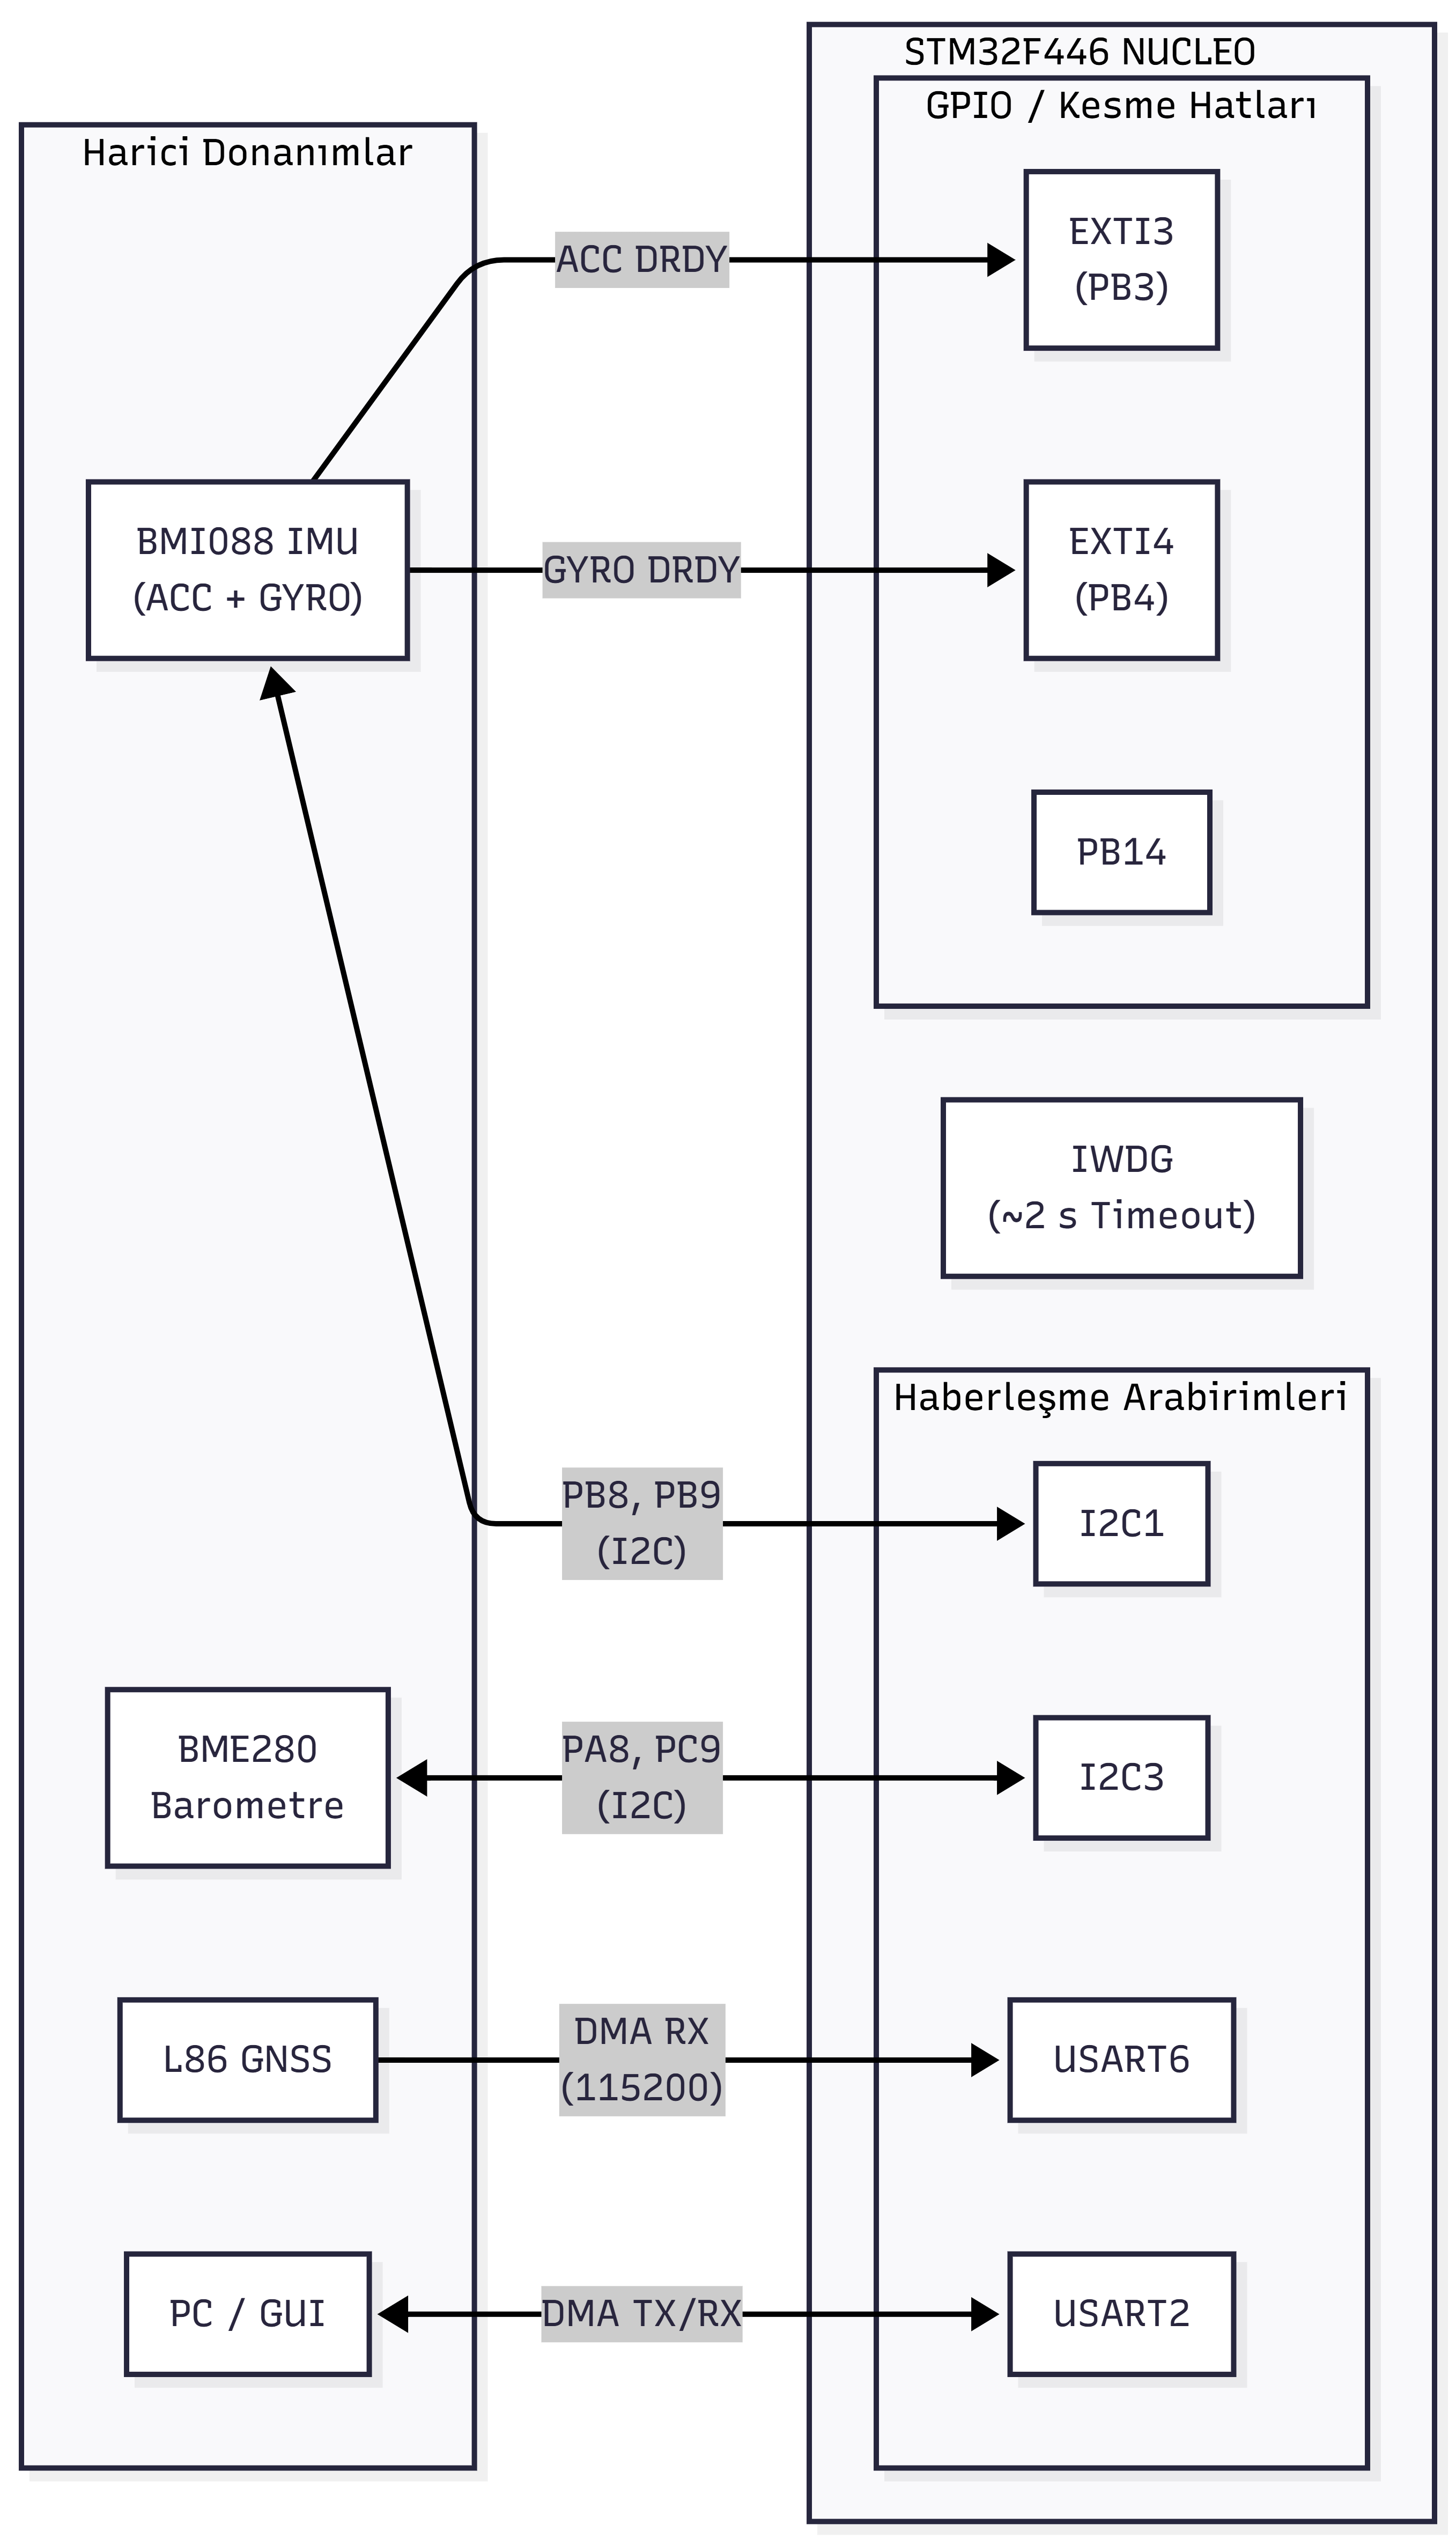
\includegraphics[width=\textwidth]{sekiller/STM32F446DonanımBlokDiyagramı.png}
    \caption{STM32F446 Donanım Blok Diyagramı ve Çevresel Birim Bağlantıları (I2C1$\rightarrow$BMI088, I2C3$\rightarrow$BME280, USART6$\rightarrow$GNSS, USART2$\rightarrow$Telemetri)}
    \label{fig:stm32f446_donanim}
\end{figure}

\subsection{Sensörler ve Ölçüm Altyapısı}
\label{sensorler_altyapisi}
Aviyonik altyapının verimli bir kestirim yapabilmesi için hassas ölçümler gerekmektedir. Sistemin dinamik davranışını okuyan ana unsurlar aşağıda belirtilmiştir:

\begin{itemize}
    \item \textbf{BMI088 (IMU):} Model roket ortamındaki yüksek ivme değişimi ve aşırı sarsıntı koşullarında güvenilir veri okumak için üretilmiş 6 eksenli bir sensördür. $\pm 24g$ ivme ölçüm aralığı ve sarsıntı altında düşük kayma (bias instability) özelliği sergileyen jiroskopu nedeniyle ivme füzyonu için seçilmiştir \cite{bosch_bmi088}. İlgili veri DMA kesmeleri üzerinden işlemciyi engellemeden koşturulur.
    \item \textbf{BME280 (Barometre):} Çevresel basıncı ölçerek Hypsometric algoritması vasıtasıyla mutlak ve bağıl irtifanın hesaplanmasını sağlayan sensördür \cite{bosch_bme280}. Ölçümleme tepki süresinin (response time) IMU sensörlerine kıyasla çok daha yavaş olması sebebiyle (10 Hz civarı), irtifa füzyonunda IMU verileri de algoritmaya katılarak Kalman filtresi destekli çift kaynaklı durum kestirimi kullanılmıştır.
    \item \textbf{L86 (GNSS):} Roketin konum koordinatlarını belirlemek adına saniyede 1 okuma (1 Hz) gerçekleştiren NMEA protokolü tabanlı GPS modülüdür. Baud hızı dinamik geçiş mekanizmaları ile USART üzerinden sürekli aralıklarla durum verisi sağlamaktadır.
\end{itemize}

\clearpage

\section{BÖLÜM: LİTERATÜR TARAMASI}
\label{literatur_taramasi}

Bu bölümde, model roket uçuş bilgisayarı ve yazılım altyapısının inşasında temel alınan bilimsel yöntemler, algoritmik yaklaşımlar ve yazılım mimarilerine yönelik literatür araştırması sunulmaktadır. Geliştirilen sistemin görev yönetimi, durum kestirimi ve uçuş kararlarının teorik altyapısı aşağıdaki alt başlıklarda detaylandırılmıştır.

\subsection{FreeRTOS Mimarisi ve Görev Yönetimi}
\label{freertos_mimarisi_ve_gorev_yonetimi}

Gerçek zamanlı bir görev yürütücüsünde (scheduler), her görev (task) çalışma anında belirli bir duruma sahiptir: \textit{Ready} (Hazır), \textit{Running} (Çalışan), \textit{Blocked} (Bloke) ve \textit{Suspended} (Askıya Alınmış) \cite{freertos_scheduler}. FreeRTOS, \textit{pxReadyTasksLists} isimli listeler üzerinden bu görevleri zamanlar. Yüksek öncelikli bir görev \textit{Ready} durumuna geçtiği an, düşük öncelikli olanı devreden çıkararak işlemciyi ele geçirir (\textit{Preemptive Multitasking}). Bu mekanizma roket yazılımlarında düşük öncelikli telemetri gönderiminin, yüksek öncelikli sensör okuma süreçlerini engellememesini güvence altına alır.

Gömülü sistemlerde Donanımsal Kesme Servis Rutinlerinden (ISR) görevlere veri iletimi, bağlam geçişinin hızını etkileyen kritik bir unsurdur. Çoklu bayrak denetimi (mutex/semaphore) yerine, bekleme süresini minimuma indiren \textit{Task Notification} yapısı kullanılmaktadır. Kesme fonksiyonu içerisinde çağrılan \verb|xTaskNotifyFromISR| ile ilgili göreve sinyal iletilir ve ardından \verb|portYIELD_FROM_ISR| makrosu sayesinde zamanlayıcı işlemciyi doğrudan hazır olan o göreve devreder \cite{freertos_tasks}. Aşağıda geliştirilen sistemde kullanılan DMA tamamlanma kesmesi ve görev bildirim mekanizması örneklendirilmiştir:

\begin{figure}[H]
    \centering
    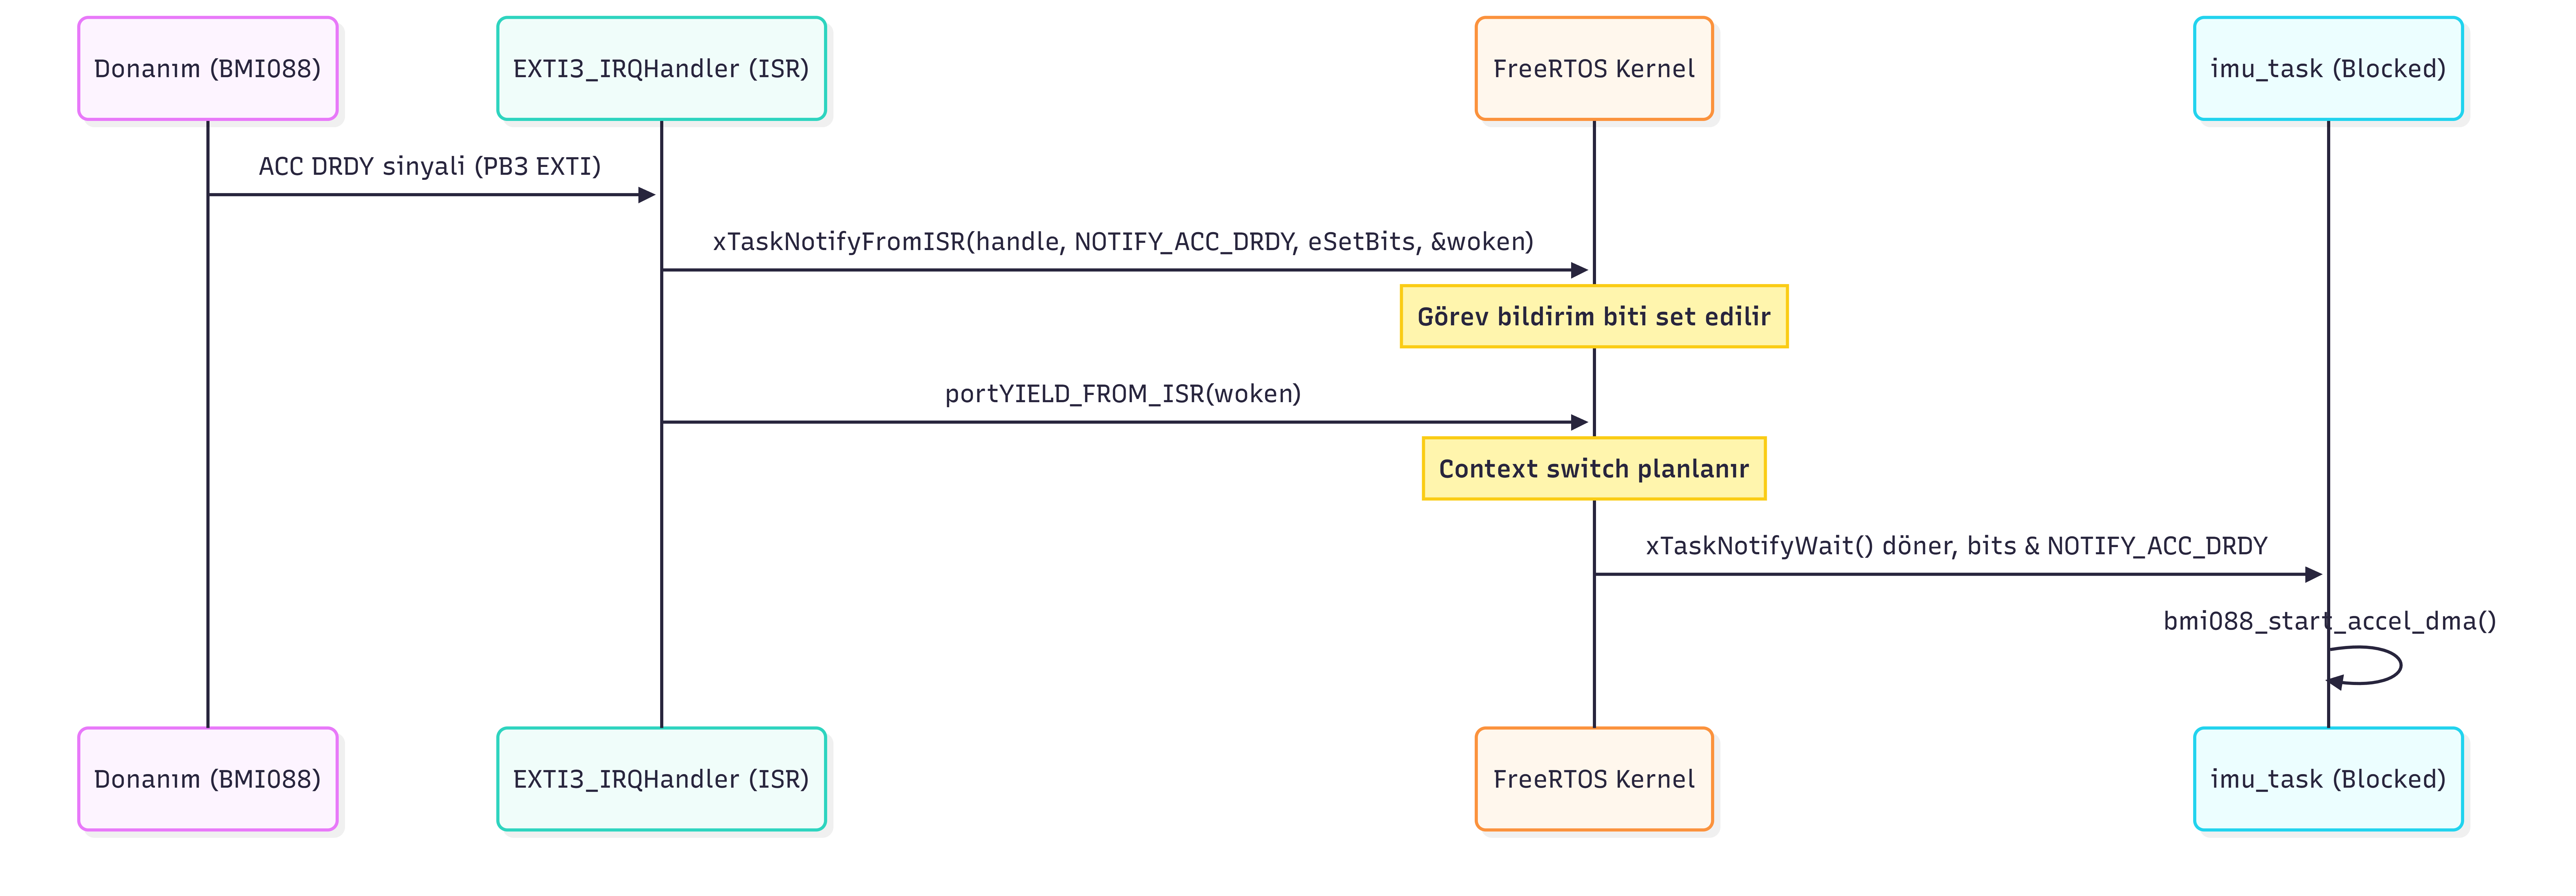
\includegraphics[width=0.8\textwidth]{sekiller/TaskNotificationKalıbı.png}
    \caption{ISR ve Task Arasında Task Notification Sinyalleşme Mimarisi}
    \label{fig:task_notification}
\end{figure}

\begin{lstlisting}[language=C, caption={Kesme Servis Rutini (ISR) İçerisinde Task Notification Kullanımı (\texttt{imu\_task.c})}]
void HAL_I2C_MemRxCpltCallback(I2C_HandleTypeDef *hi2c)
{
    if (hi2c->Instance != I2C1 || s_handle == NULL) return;

    BaseType_t woken = pdFALSE;
    xTaskNotifyFromISR(s_handle, NOTIFY_DMA_DONE, eSetBits, &woken);
    portYIELD_FROM_ISR(woken); // Eger imu_task hazir ise aninda baglam degistir
}
\end{lstlisting}

Görevler arası durum paylaşımı (Snapshot mekanizması) için Derinliği 1 (\textit{depth=1}) olan kuyruklar (Queue mailbox pattern) tercih edilmiştir. \verb|xQueueOverwrite| kullanılarak eski veri silinip sürekli yeni uçuş verisi yazılır (Producer) ve diğer görevler tarafından eksiltme olmadan kopyası alınabilmesi için \verb|xQueuePeek| fonksiyonu kullanılır (Consumer) \cite{freertos_queue}. Kuyruk derinliğinin 1 olması, bellekte gereksiz tamponlama (buffering) yapılmasını engelleyerek her görevin son uçuş durumuna erişmesini garanti etmektedir.

\begin{figure}[H]
    \centering
    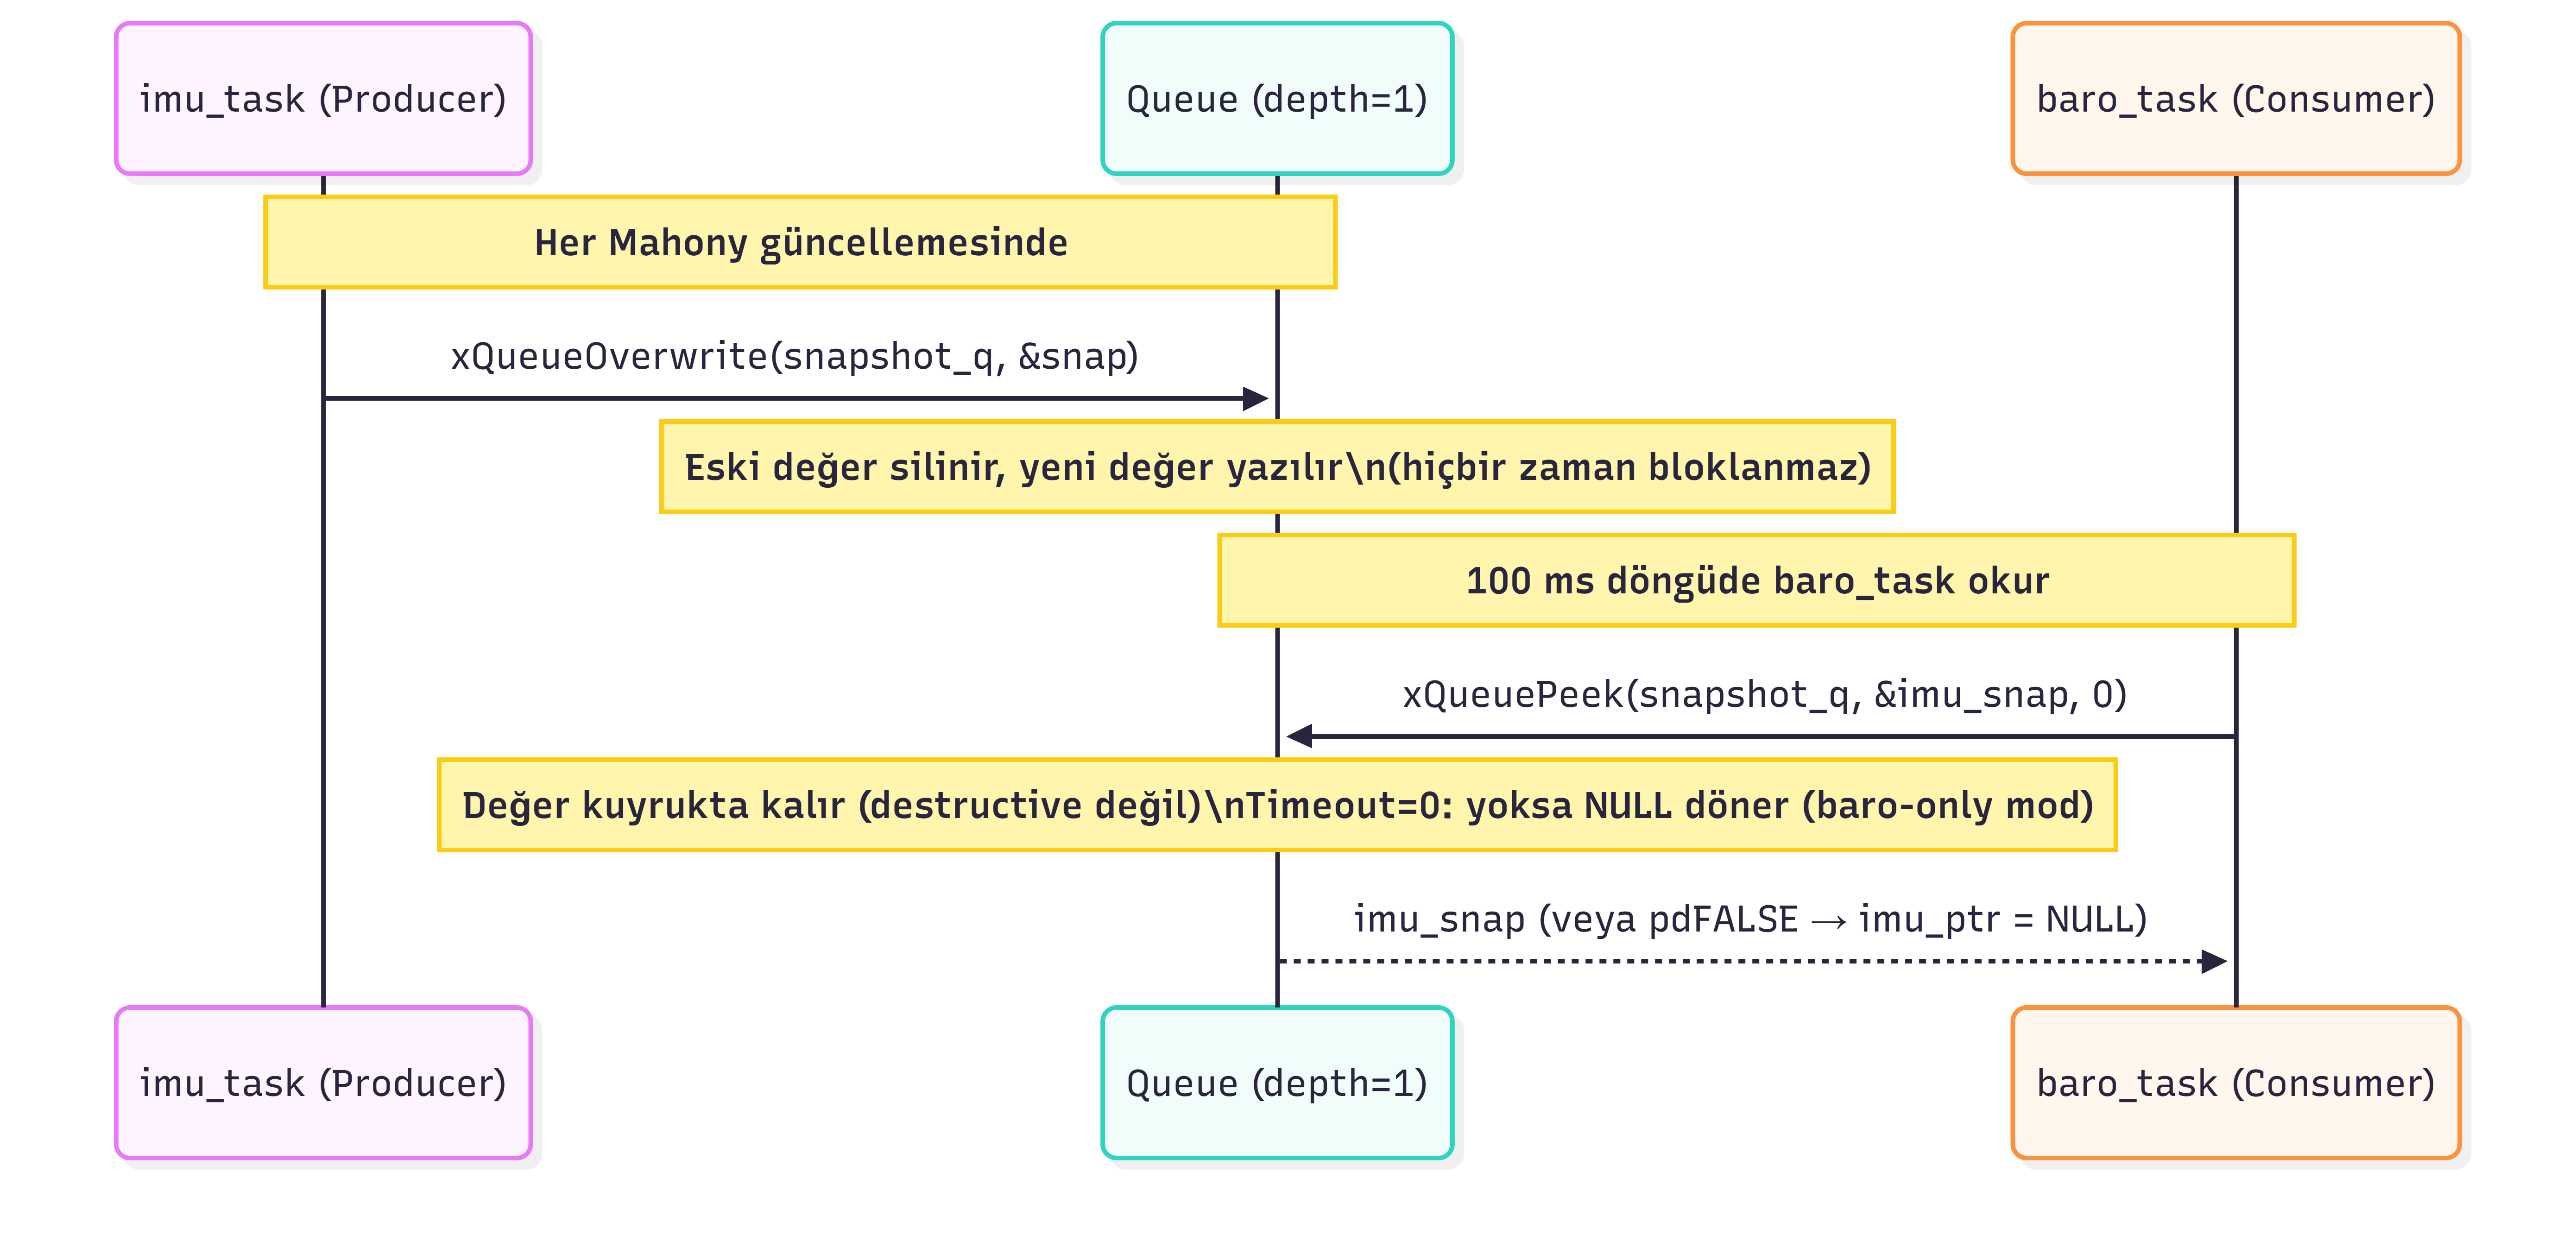
\includegraphics[width=0.8\textwidth]{sekiller/TaskSnapshotQueueKalıbı.png}
    \caption{Görevler Arası Derinliği 1 Olan Kuyruk (Snapshot Queue) Veri Paylaşım Kalıbı}
    \label{fig:task_snapshot}
\end{figure}

\subsection{Sensör Füzyonu Yöntemleri (Mahony, Kalman)}
\label{sensor_fuzyonu_yontemleri}

Roketlerin fırlatma anı esnasında maruz kaldığı şiddetli titreşimler ve motor ivmesi, salt ivmeölçer verisini son derece gürültülü hale getirir. Diğer yandan jiroskoplar gürültüden daha az etkilense de, zamanla küçük sapmaların matematiksel bütünleştirilmesi dolayısıyla kayma hatası (drift) üretir. Bu nedenle füzyon işlemi zorunludur \cite{stanford_imu_notes}. Geleneksel \textit{Tamamlayıcı Filtre} (Complementary Filter) yaklaşımı, jiroskopun kısa dönem kararlılığı ile ivmeölçerin uzun dönem doğruluğunu;

\begin{equation}
\theta_{t} = \alpha \left( \theta_{t-1} + \omega \Delta t \right) + (1 - \alpha)\theta_{acc}
\end{equation}

denklemiyle birleştirir \cite{ahrs_doc}, fakat bu fırlatma esnasındaki eksen kaymalarında yetersiz kalmaktadır. Projede Euler açı açmazını (Gimbal Lock) ortadan kaldıran ve oransal-integral (PI) hata geri beslemesi mantığıyla çalışan \textbf{Mahony Filtresi} tercih edilmiştir \cite{ahrs_mahony_doc, madgwick2011estimation}. Burada yerçekimi tahmin vektörü $\hat{\mathbf{g}}$ ile normalize edilen tahmini ivme vektörü $\mathbf{a}_{norm}$ arasındaki hata ($e$) Vektörel Çarpım yoluyla belirlenir:

\begin{equation}
\mathbf{e} = \hat{\mathbf{g}} \times \mathbf{a}_{norm}
\end{equation}

Bu hata hesaplandıktan sonra, Quaternion ($q$) entegrasyonu; jiroskop ölçümleri, jiroskop sapmasını dengeleyen entegrasyon terimi ($\mathbf{b}$) ve hata ($e$) vektörünün katılması ile sürekli yenilenmektedir:

\begin{equation}
\dot{q} = \frac{1}{2} q \otimes \left( \omega_{gyro} - \mathbf{b} + K_p \mathbf{e} + K_i \int \mathbf{e} \, dt \right)
\end{equation}

İrtifa Füzyonu aşamasında ise sistemdeki \textit{Baro (BME280)} ile \textit{IMU (Z ekseni)} entegrasyonu \textbf{Kalman Filtresi} aracılığıyla gerçekleştirilmektedir \cite{welch1995introduction}. Kalman filtresinde durum vektörü $\hat{x}_k = [ \text{İrtifa}, \text{Hız}, \text{İvme\_Bias} ]^T$ şeklinde konumlandırılmıştır. Sabit ivme kullanılarak varsayılan durum geçiş matrisi ($F$):

\begin{equation}
\hat{x}_{k|k-1} = F \hat{x}_{k-1|k-1} + B \cdot u_{k}  \quad , \quad
P_{k|k-1} = F P_{k-1|k-1} F^T + Q
\end{equation}

Denklemlerde belirtilen $Q$ süreç (process) gürültüsünü, hesaplanan barometre verilerindeki gürültü kovaryans matrisi $R$ ise ölçüm gürültüsünü ifade eder. İkinci adımda kazanç ($K$) oluşturulur ve gözlem matrisi ($H$) ile ölçülen veri kullanılarak yapı güncellenir:

\begin{equation}
K_k = P_{k|k-1} H^T (H P_{k|k-1} H^T + R)^{-1}
\end{equation}

\begin{equation}
\hat{x}_{k|k} = \hat{x}_{k|k-1} + K_k (z_k - H \hat{x}_{k|k-1})
\end{equation}

\subsection{Uçuş Durum Makinesi Yaklaşımları}
\label{ucus_durum_makinesi_yaklasimlari}

Bir roketin kalkış öncesinden yere inene değin geçen fazları algoritmik bir biçimde idare edebilmek için Durum Makinesi (Finite State Machine - FSM) konseptleri öne çıkmaktadır. Literatürde güvenilirliği sağlamak amacıyla FSM mimarileri kullanılmaktadır; çünkü bu tasarımlar \textit{if-else} spagetti kod karmaşasını önler, olaylar arası tetikleyicilerin izlenebilirliğini (traceability) artırır ve roket kurtarma fırlatmalarının yanlış fazlarda gerçekleşmesini izole eder. 

Model roket projelerinde literatür çerçevesinde tanımlanmış ve geliştirilmiş temel operasyon fazları: IDLE (Hazır Bekleme), BOOST (Kalkış İvmelenmesi), COAST (Serbest Uçuş/Süzülme), APOGEE (Tepe Noktası - Drogue Paraşütü), DROGUE\_DESCENT (1. Aşama İniş), MAIN\_DESCENT (2. Aşama Ana Paraşüt İnisi) ve LANDED (Yere İniş) adımlarından oluşmaktadır. Apogee (Tepe Noktası) tespit algoritmalarında yaşanabilecek yanılmaların önüne geçmek adına çoklu tepe noktası mekanizmaları tanımlanmıştır; \textit{hız bazlı apogee} (Kalman filtresinden gelen düşey hız vektörünün 0'ın altına inmesi) ile yönelime duyarlı \textit{tilt bazlı apogee} (Mahony tahmini Pitch açısının (theta) 70$^\circ$'nin üzerine çıkması). Bu iki şarttan birinin tetiklenmesiyle sistem duruma otomatik olarak geçiş yapmaktadır.

\clearpage
\section{BÖLÜM: SİSTEM MİMARİSİ VE YÖNTEM}
\label{bolum3}

Bu bölümde model roket uçuş bilgisayarı için tasarlanan yazılımsal ve donanımsal mimarinin detayları sunulmaktadır. Sistemin katmanlı yapısı, donanım birimlerinin kullanımı ve FreeRTOS eksenindeki görev mimarisi açıklanmıştır.

\subsection{Katmanlı Yazılım Mimarisi}
\label{katmanli_yazilim_mimarisi}

Model roketin aviyonik yazılım sistemi, modülerliğin sağlanması ve donanım bağımlılığının en aza indirilmesi amacıyla 4 temel katmandan (Donanım, HAL, Sürücü/Middleware, Uygulama) oluşacak şekilde tasarlanmıştır. Her katman yalnızca kendi altındaki katmanlar ile iletişim kuracak şekilde (tek yönlü bağımlılık ilkesi) yapılandırılmıştır.

\begin{itemize}
    \item \textbf{Donanım Katmanı (Hardware):} STM32F446 mikrodenetleyicisi, sensörler (BMI088, BME280, L86) ve iletişim yolları (I2C, SPI, USART).
    \item \textbf{HAL Katmanı (Hardware Abstraction Layer):} STMicroelectronics tarafından sağlanan ve STM32CubeMX ile otomatik üretilen bu katman, donanım kayıtçılarının (register) doğrudan manipüle edilmesi yerine standart API'ler sunar. Uçuş güvenilirliği için CubeMX tarafından \textit{Core/Src/} altında oluşturulan `gpio.c`, `i2c.c` gibi başlatma kodlarına dışarıdan müdahale edilmemiş, tüm işlevsellik kullanıcı dosyalarında gerçeklenmiştir.
    \item \textbf{Sürücü/Middleware Katmanı:} FreeRTOS işletim sistemi çekirdeği ile birlikte sensörlerin (BME280, BMI088 vb.) spesifik konfigürasyonlarını içeren sürücü dosyalarını barındırır.
    \item \textbf{Uygulama Katmanı (Application):} Uçuş algoritmalarının, sensör füzyonunun (Mahony, Kalman) ve tepe noktası tayini gibi uçuş fazlarını idare eden operasyonel görevlerin (Tasks) bulunduğu en üst katmandır.
\end{itemize}

\begin{figure}[H]
    \centering
    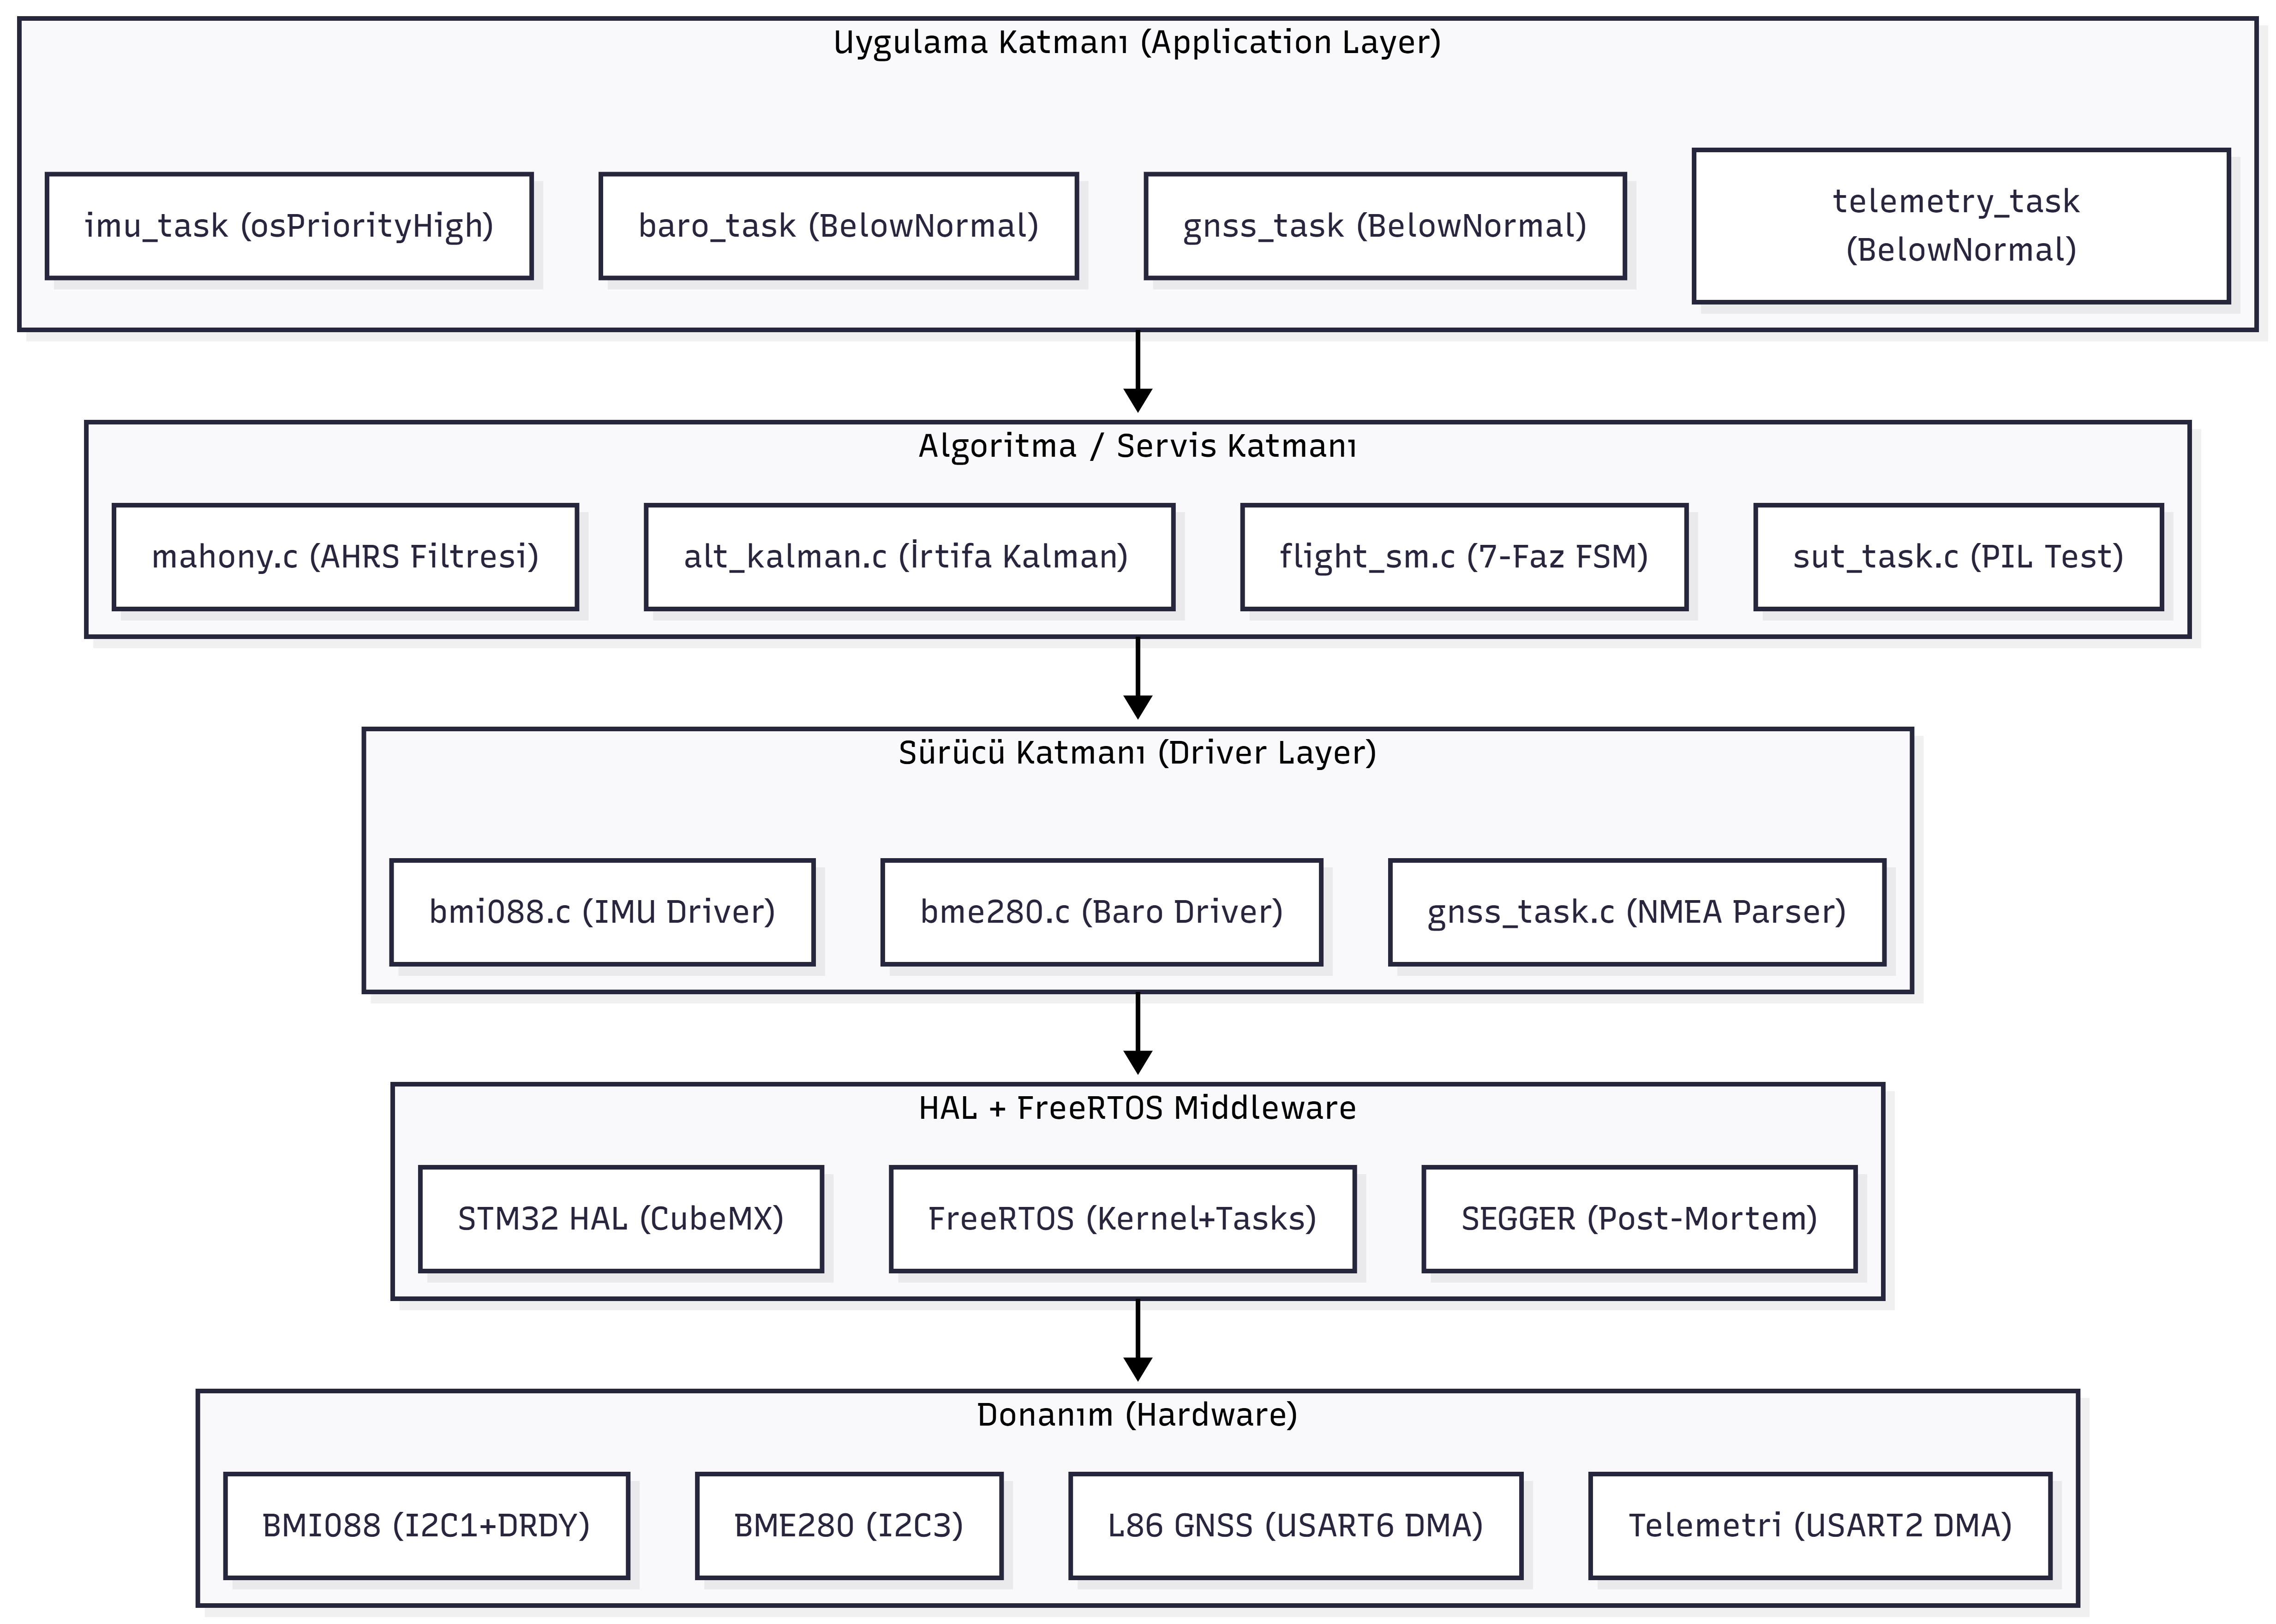
\includegraphics[width=0.8\textwidth]{sekiller/KatmanlıYazılımMimarisi(4 katman).png}
    \caption{Uçuş Bilgisayarı 4 Katmanlı Yazılım Mimarisi ve SIT/SUT Entegrasyonu}
    \label{fig:katmanli_mimari}
\end{figure}

\subsection{Donanım Haritası ve Çevresel Birimler}
\label{donanim_haritasi}

Uçuş algoritmasının ihtiyaç duyduğu verilerin toplanabilmesi için mikrodenetleyicinin çevresel birimleri spesifik görevlere atanmıştır. Haberleşme birimlerinde işlemciyi (CPU) meşgul etmemek adına Doğrudan Bellek Erişimi (DMA) mimarisi uygulanmıştır. BME280 sensörü I2C3, BMI088 (İvmeölçer ve Jiroskop) ise I2C1 veri yolları üzerinden sisteme bağlanmıştır. Ayrıca veri hazır kesmesini asenkron olarak tetiklemek için EXTI (Dış Kesme) hatları kullanılmıştır.

Sistemin, elektromanyetik parazitler veya olası bir yazılımsal döngü tıkanıklığı (deadlock) karşısında kilitlenmemesi adına Donanımsal Bağımsız Zamanlayıcı (IWDG - Independent Watchdog) kurulmuştur. IWDG yapılandırmasında frekans bölücü (prescaler) değeri 256, yeniden yükleme (reload) değeri ise 249 olarak atanmış olup yaklaşık 2 saniyelik bir \textit{timeout} (zaman aşımı) süresi sağlanmıştır. Belirtilen bu süre içinde barometre görevi Watchdog'u beslemezse (yenilemezse), donanım otomatik olarak sistem sıfırlaması (reset) uygular.

\begin{table}[htbp]
    \centering
    \caption{Donanım Haritası ve Çevresel Birim Görevleri}
    \label{tab:donanim_haritasi}
    \begin{tabular}{|l|l|l|l|}
    \hline
    \textbf{Çevresel Birim} & \textbf{Pin Ataması} & \textbf{Protokol} & \textbf{Sorumlu Görev / Modül} \\ \hline
    I2C1 & PB8 (SCL), PB9 (SDA) & I2C (Hızlı Mod) & BMI088 (İvme \& Jiroskop) \\ \hline
    I2C3 & PA8 (SCL), PC9 (SDA) & I2C (Standart Mod) & BME280 (Barometre) \\ \hline
    EXTI3 & PB3 & GPIO Kesmesi & BMI088 İvme DRDY Sinyali \\ \hline
    EXTI4 & PB4 & GPIO Kesmesi & BMI088 Jiroskop DRDY Sinyali \\ \hline
    USART6 & DMA RX & Seri Haberleşme & GNSS (L86) Modülü \\ \hline
    USART2 & DMA TX/RX & Seri Haberleşme & Telemetri (SIT / ST-Link VCP) \\ \hline
    IWDG & Dahili (LSI) & - & Donanımsal Hata Koruması \\ \hline
    BUZZER & PB14 & GPIO & Durum ve Uyarı Sinyali \\ \hline
    \end{tabular}
\end{table}

\subsection{FreeRTOS Görev Mimarisi}
\label{freertos_gorev_mimarisi}

Operasyonel kısıtlar doğrultusunda FreeRTOS mimarisi üzerinde birbirini kesebilen ve durum önceliklerine göre sıralanmış toplam dört yapısal görev (Task) tasarlanmıştır. SUT (System Under Test) modunda donanımsal sensör okuması yapılmadığından, IMU, Baro, GNSS ve Telemetri görevleri \verb|vTaskDelay| ile uyku döngülerinde tutularak \textit{sut\_task} modülüne alan açmaktadır.

Gerçek donanım modunda; ISR'dan başlayan sensör tetiklemeleri bir zincirleme aksiyon üretir. Bu deterministik akış: DRDY (Data Ready) Pin $\rightarrow$ EXTI ISR $\rightarrow$ \verb|xTaskNotifyFromISR| $\rightarrow$ IMU görevi uyanması $\rightarrow$ DMA transferini başlatması $\rightarrow$ Tamamlanma (DMA Complete) Kesmesi $\rightarrow$ Parse işlemi $\rightarrow$ Snapshot Güncellemesi şeklinde işletilir.

Snapshot mekanizması, görevlerin \textit{veriye tek kaynaklı dönüşümünü} garanti altına almak için Derinliği 1 (\textit{depth=1}) boyutunda olan FreeRTOS kuyruklarıyla inşa edilmiştir. Yığın (Stack) bellek taşmalarına karşı FreeRTOS konfigürasyonunda \verb|configCHECK_FOR_STACK_OVERFLOW| seviyesi 2'ye çekilmiştir.

\begin{table}[htbp]
    \centering
    \caption{FreeRTOS Görev Öncelikleri ve Temel Özellikleri}
    \label{tab:gorev_tablosu}
    \begin{tabular}{|l|l|p{1.5cm}|p{3.5cm}|p{3cm}|}
    \hline
    \textbf{Görev Adı} & \textbf{Öncelik} & \textbf{Stack (Byte)} & \textbf{Tetikleyici} & \textbf{İşlem / Periyot} \\ \hline
    imu\_task & osPriorityHigh & $512 \times 4$ & Donanım Kesmesi & Mahony, Snapshot \\ \hline
    baro\_task & osPriorityBelowNormal & $512 \times 4$ & 100 ms Periyot & Kalman, Flight SM \\ \hline
    gnss\_task & osPriorityBelowNormal & $512 \times 4$ & DMA Circular RX & 1 Hz NMEA Parse \\ \hline
    telemetry\_task & osPriorityBelowNormal & $256 \times 4$ & İletişim Hazır & 50 Hz UART Gönderimi \\ \hline
    \end{tabular}
\end{table}

Aşağıdaki kod parçasında, ivme veya jiroskop kesmelerinden (\textit{notify}) uyanan IMU görevinin DMA işlem zincirini (StateMachine) yönetmesi gösterilmektedir:

\begin{lstlisting}[language=C, caption={IMU Görevi İçerisindeki DMA Durum Makinesi Yönetimi}]
if (dma_state == DMA_IDLE) {
    if (acc_pending) {
        if (bmi088_start_accel_dma(k_bmi_cfg.hi2c, s_acc_buf) == HAL_OK) {
            dma_state   = DMA_READING_ACC;
            acc_pending = false;
        }
    } else if (gyro_pending) {
        if (bmi088_start_gyro_dma(k_bmi_cfg.hi2c, s_gyro_buf) == HAL_OK) {
            dma_state    = DMA_READING_GYRO;
            gyro_pending = false;
        }
    }
}
\end{lstlisting}

\subsection{Sensör Sürücüleri}
\label{sensor_suruculeri}

\subsubsection{BMI088 IMU Sürücüsü (I2C + DMA + DRDY IRQ)}
Veri toplama mimarisinin temeli olan BMI088 İvmeölçer ve Jiroskop sensörü, mimari yapısı gereği sistemde hız kısıtı oluşturmaması için iki ayrı donanım adresi halinde ele alınmıştır. İlgili veri okuma süreci tamamıyla kesme tabanlı asenkron bir yöntemle sağlanmaktadır:

\begin{itemize}
    \item \textbf{DRDY (Data Ready) Pin Tetiklemesi:} Her iki sensörden gelen (İvme EXTI3, Jiroskop EXTI4) veri hazır pinleri donanımsal kesme (Interrupt) fonksiyonunu tetikler.
    \item \textbf{DMA Non-blocking Okuma:} \verb|bmi088_start_accel_dma| fonksiyonu kullanılarak işlemci işgal edilmeden veriler bellek adreslerine çekilir.
    \item \textbf{Anlamlı Veriye (Parse) Dönüştürme:} $\pm 12g$ olarak alınan ivme aralığı \verb|bmi088_parse_accel| komutu ile $m/s^2$'ye çevrilir; 2000 dps aralığındaki jiroskop verisi rad/s birimine dönüştürülür.
\end{itemize}

\begin{figure}[H]
    \centering
    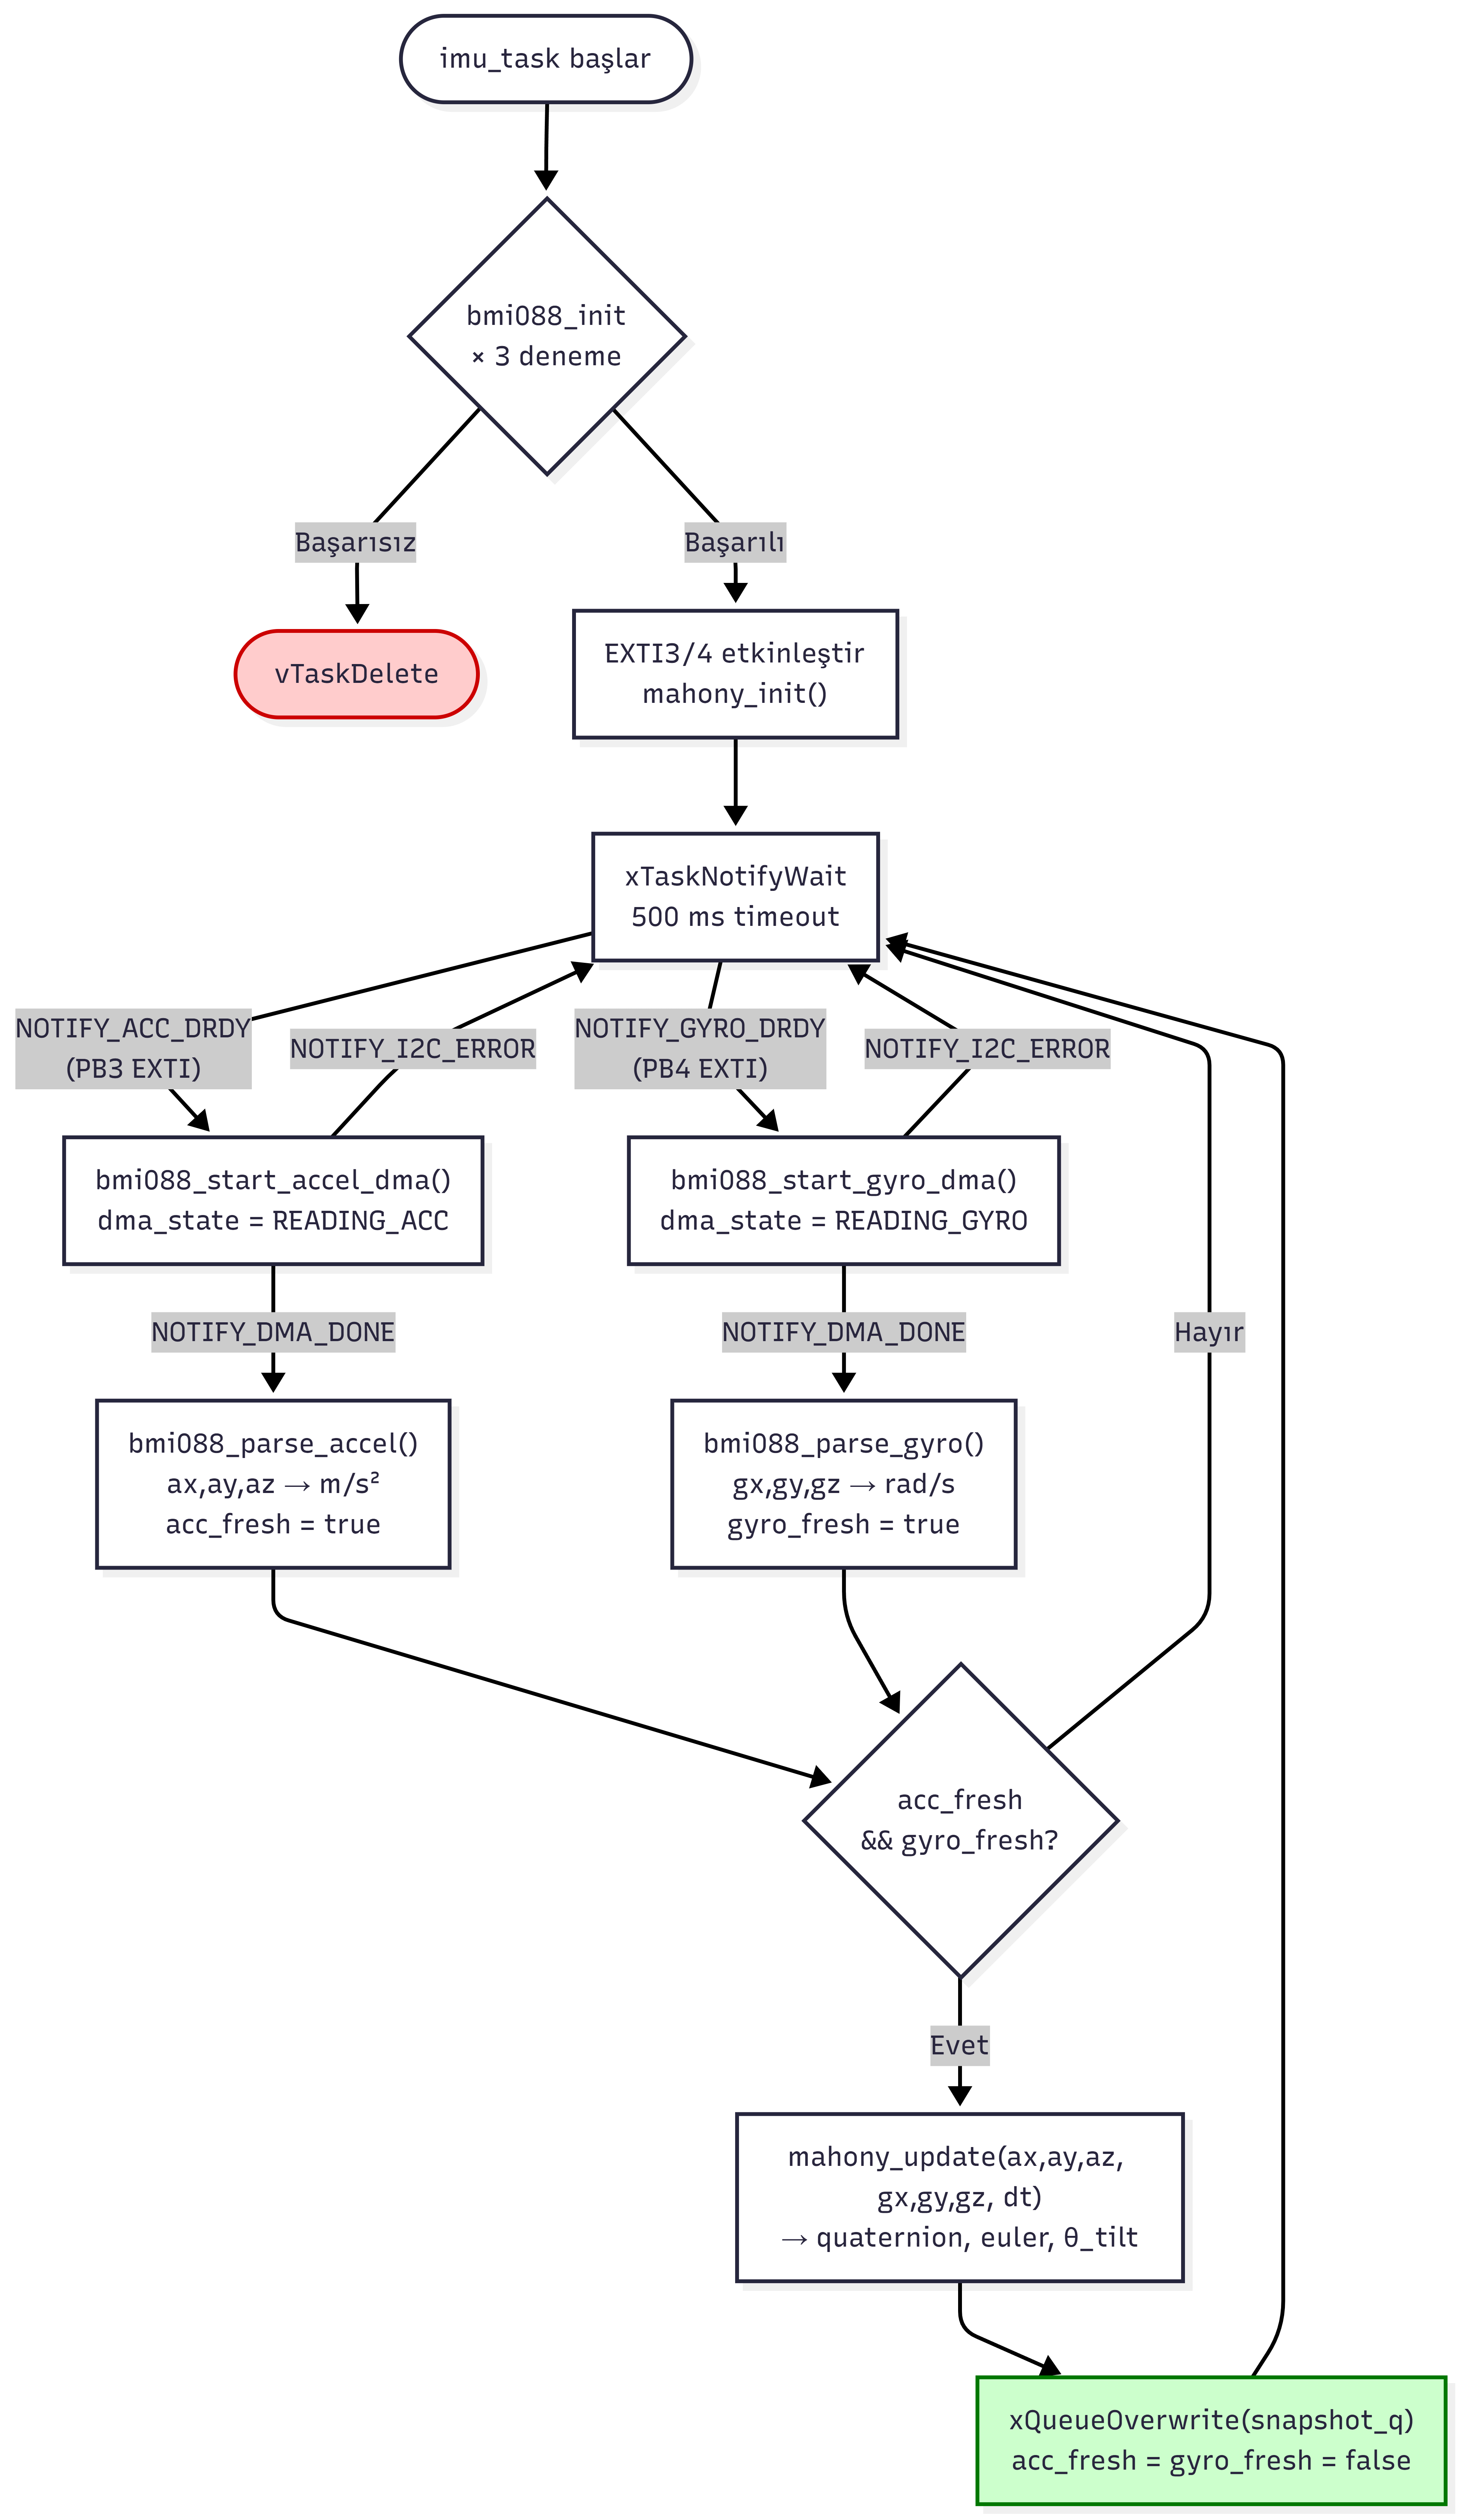
\includegraphics[width=\textwidth]{sekiller/IMU_Pipeline.png}
    \caption{BMI088 IMU Veri İşleme Hattı (Pipeline) ve Mahony Entegrasyonu}
    \label{fig:imu_pipeline}
\end{figure}

Başlangıç aşamasında meydana gelebilecek iletişim hatalarına karşı 3 denemeli bir tekrar (\textit{retry}) döngüsü kurgulanmıştır. Başarısızlık durumunda yazılım baro-only (sadece barometre) modunda çalışmaya devam etmek üzere ilgili görevi FreeRTOS üzerinden siler.

\begin{lstlisting}[language=C, caption={BMI088 İletişim Başlangıç ve Retry Döngüsü (\texttt{imu\_task.c})}]
int retries = 3;
while (bmi088_init(&k_bmi_cfg) != 0) {
    if (--retries == 0) {
        vTaskDelete(NULL); // Sensor yok, gorevi sil
        return;
    }
    HAL_I2C_DeInit(&hi2c1);
    __HAL_RCC_I2C1_FORCE_RESET();
    vTaskDelay(pdMS_TO_TICKS(10));
    __HAL_RCC_I2C1_RELEASE_RESET();
    vTaskDelay(pdMS_TO_TICKS(10));
    MX_I2C1_Init();
    vTaskDelay(pdMS_TO_TICKS(30));
}
\end{lstlisting}

\subsubsection{BME280 Barometrik Basınç Sürücüsü}
Sistemdeki barometrik basınç verisi I2C3 yolu üzerinden saniyede 10 örnek (10 Hz) alınacak şekilde tasarlanmıştır. \verb|vTaskDelayUntil| fonksiyonu kullanılarak, görevin her koşulda 100 ms periyot kısıtına uyması (\textit{catch-up}) güvence altına alınmıştır. 

Sensör üzerinden ham olarak alınan basınç ve sıcaklık verisi Bosch datasheet katsayılarına göre kompanze edilip irtifaya çevrilmektedir. İrtifa referans kalibrasyonu (boot evresinde alınan ilk değer) referans noktası kabul edilerek roketin yerden yüksekliği saptanır. Görev sonrasında ise sırasıyla \verb|alt_kalman_update| tetiklenerek hız-ivme kestirimi tamamlanır ve \verb|flight_sm_update| adımına girilir. Barometre döngüsünün ekseni şu şekildedir:

\begin{figure}[H]
    \centering
    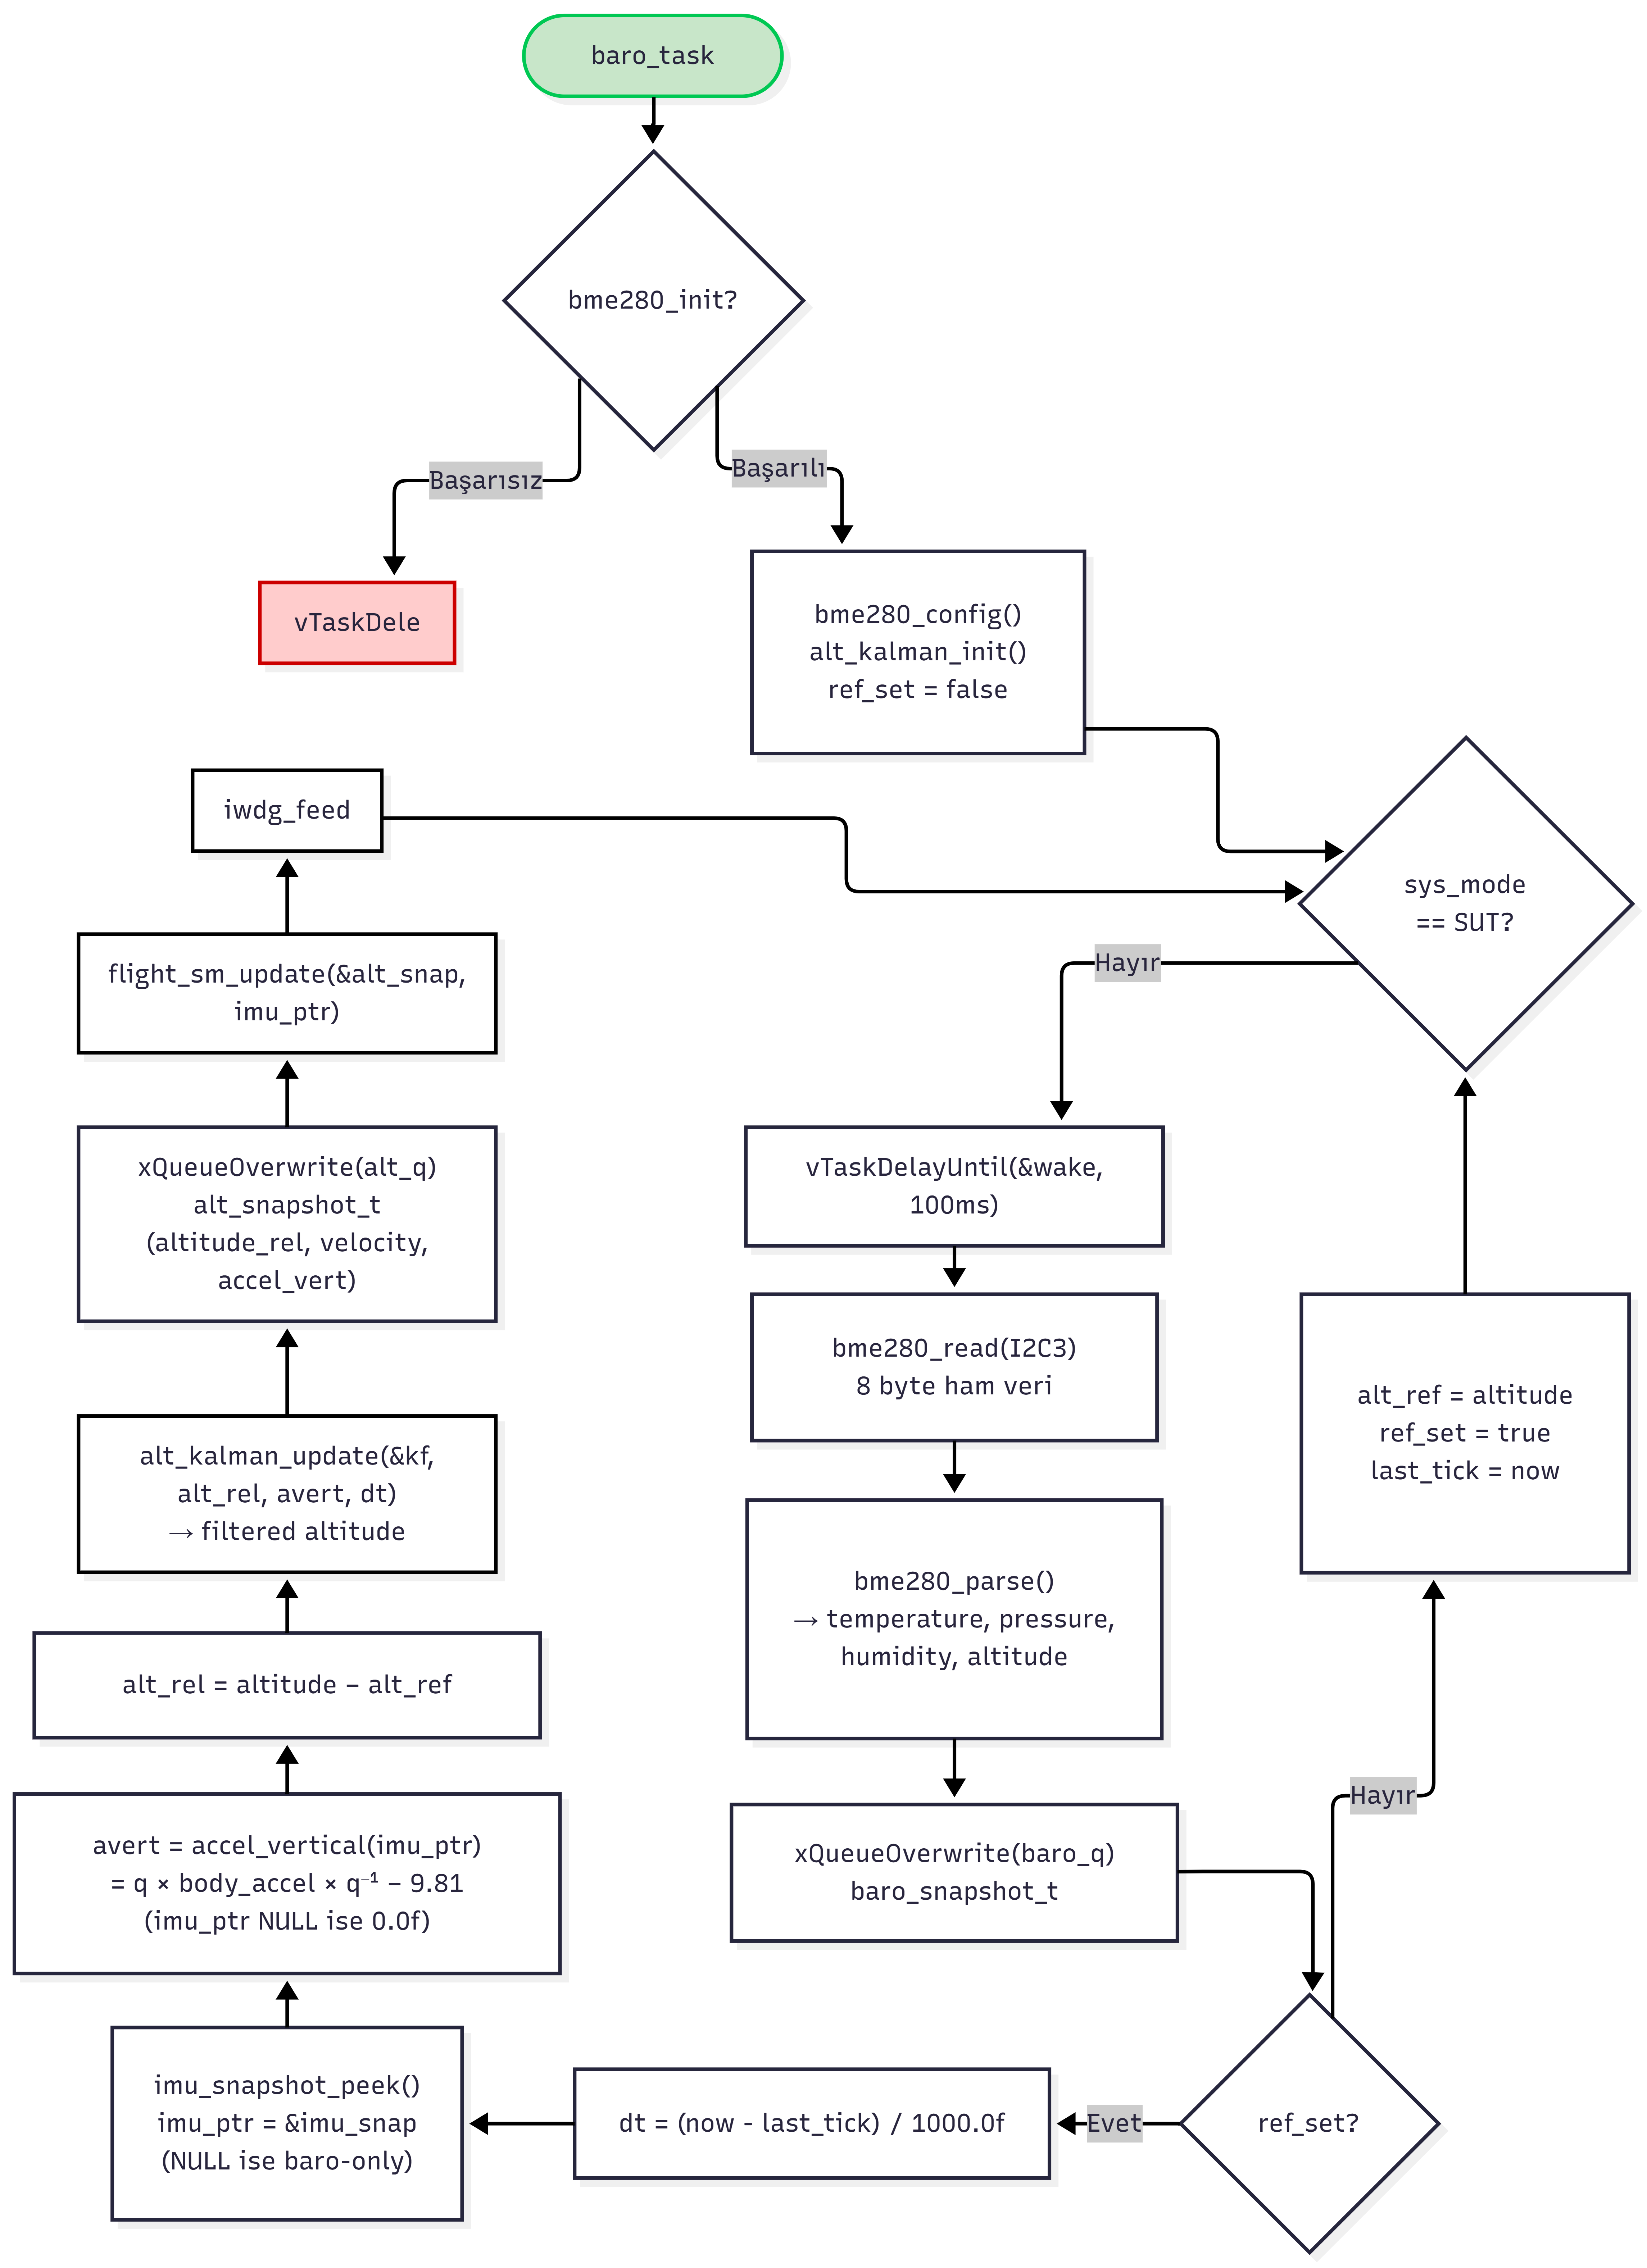
\includegraphics[width=\textwidth]{sekiller/Baro TaskAnaDöngüsü_veKalman_entegrasyonu.png}
    \caption{Barometre Ana Döngüsü, Kalman Filtresi ve FSM Entegrasyonu}
    \label{fig:baro_pipeline}
\end{figure}

\begin{lstlisting}[language=C, caption={10 Hz Barometre Okuma, Kalman ve Uçuş FSM Akışı (\texttt{baro\_task.c})}]
uint8_t raw[8];
if (bme280_read(&hi2c3, raw) != HAL_OK) continue;

bme280_parse(raw, &calib, &data);

float alt_rel  = data.altitude - alt_ref;
float filtered = alt_kalman_update(&kf, alt_rel, avert, dt);

flight_sm_update(&alt_snap, imu_ptr);
\end{lstlisting}

\subsubsection{L86 GNSS Modülü (Circular DMA, NMEA)}
Konum verisi, işlemci müdahalesi olmaksızın arabelleklerin kesintisiz dolmasını sağlayan Circular (Dairesel) DMA RX modeli kullanılarak USART6 üzerinden işlenmektedir. \verb|GNSS_BUF_HALF| arabelleğinin alt ve üst seviyesi dolduğunda ayrı yarı-kesmeler oluşturularak (\verb|0x01U|, \verb|0x02U|) NMEA katarı (\verb|GNRMC|, \verb|GPGGA|) \verb|sscanf| ile incelenip enlem, boylam, hız ve HDOP gibi argümanlar parçalanmaktadır.
Sistem başlarken L86 standart baud hızı olan 9600 bps seviyesinden \verb|$PMTK251| komutuyla 57600 bps geçişine ayarlanır. Veriler saniyede 1 kere (1 Hz) snapshot dosyasına yüklenir. Eğer GNSS sinyali uydulardan fix bulamazsa \verb|is_valid| bayrağı kapalı tutularak karar mekanizmalarının yanıltılması engellenmektedir.

\subsection{Sensör Füzyonu ve Durum Kestirimi}
\label{sensor_fuzyonu_ve_durum_kestirimi}

\subsubsection{Mahony AHRS Filtresi (6DOF Quaternion)}
Model roketin 3 boyutlu uzayda Euler açısı problemlerini (Gimbal Lock) devreden çıkarmak amacıyla hesaplama süreçlerinde \textit{Quaternion} formülasyonu kullanılmıştır. Mahony filtresinin öncelikli adımı normalize edilmiş ivme ile quaternion destekli tahmini yerçekiminin hatalarını çıkarıp ($\mathbf{e} = \hat{\mathbf{g}} \times \mathbf{a}_{norm}$) PI denetleyicisi ile sisteme dahil etmektir. 

Verimli işlem performansı için Quake III "Fast Inverse Square Root" (\verb|inv_sqrt|) kullanılarak ağırlık hafifletilmiştir. Kod içerisinde oransal kazanç ($K_p=2.0$) ve integral kazancı ($K_i=0.005$) olarak ele alınmıştır. Çıkan 6 eksen quaternion hesabı sırasıyla roll, pitch, yaw ve \textit{theta (eğim açısı)} verilerine dönüştürülür.

\begin{lstlisting}[language=C, caption={Mahony Quaternion Türevi Güncellemesi (\texttt{mahony.c})}]
/* Jiroskop hata duzeltmesi ve quaternion turevi */
float gx_corr = gx + m->twoKp * ex + m->integral[0];
float gy_corr = gy + m->twoKp * ey + m->integral[1];
float gz_corr = gz + m->twoKp * ez + m->integral[2];

float qDot1 = 0.5f * (-q2 * gx_corr - q3 * gy_corr - q4 * gz_corr);
float qDot2 = 0.5f * ( q1 * gx_corr + q3 * gz_corr - q4 * gy_corr);
/* ... diger quaternion carpimlari ve entegrasyon */
\end{lstlisting}

\subsubsection{Yükseklik Kalman Filtresi (Baro + IMU)}
Barometre ve IMU'dan elde edilen birbirinden farklı zemin karakteristiğine sahip iki veriyi optimum düzeyde birleştirmek için 3 boyutlu durum vektörüne sahip ($x = [\text{irtifa}, \text{hız}, \text{ivme\_bias}]^T$) geliştirilmiş yükseklik Kalman filtresi uyarlanmıştır. Filtrenin sistem geçiş ($F$), ölçüm modeli ($H$) ile zamanın karesel artış parametreleri ($Q$) tanımlanmıştır:

\begin{equation}
F = \begin{bmatrix}
1 & \Delta t & \Delta t^2/2 \\
0 & 1 & \Delta t \\
0 & 0 & 1
\end{bmatrix} \quad , \quad
H = \begin{bmatrix}
1 & 0 & 0 \\
0 & 0 & 1
\end{bmatrix} \quad , \quad
Q = q \begin{bmatrix}
\frac{\Delta t^4}{4} & \frac{\Delta t^3}{2} & \frac{\Delta t^2}{2} \\
\frac{\Delta t^3}{2} & \Delta t^2 & \Delta t \\
\frac{\Delta t^2}{2} & \Delta t & 1
\end{bmatrix}
\end{equation}

\begin{figure}[H]
    \centering
    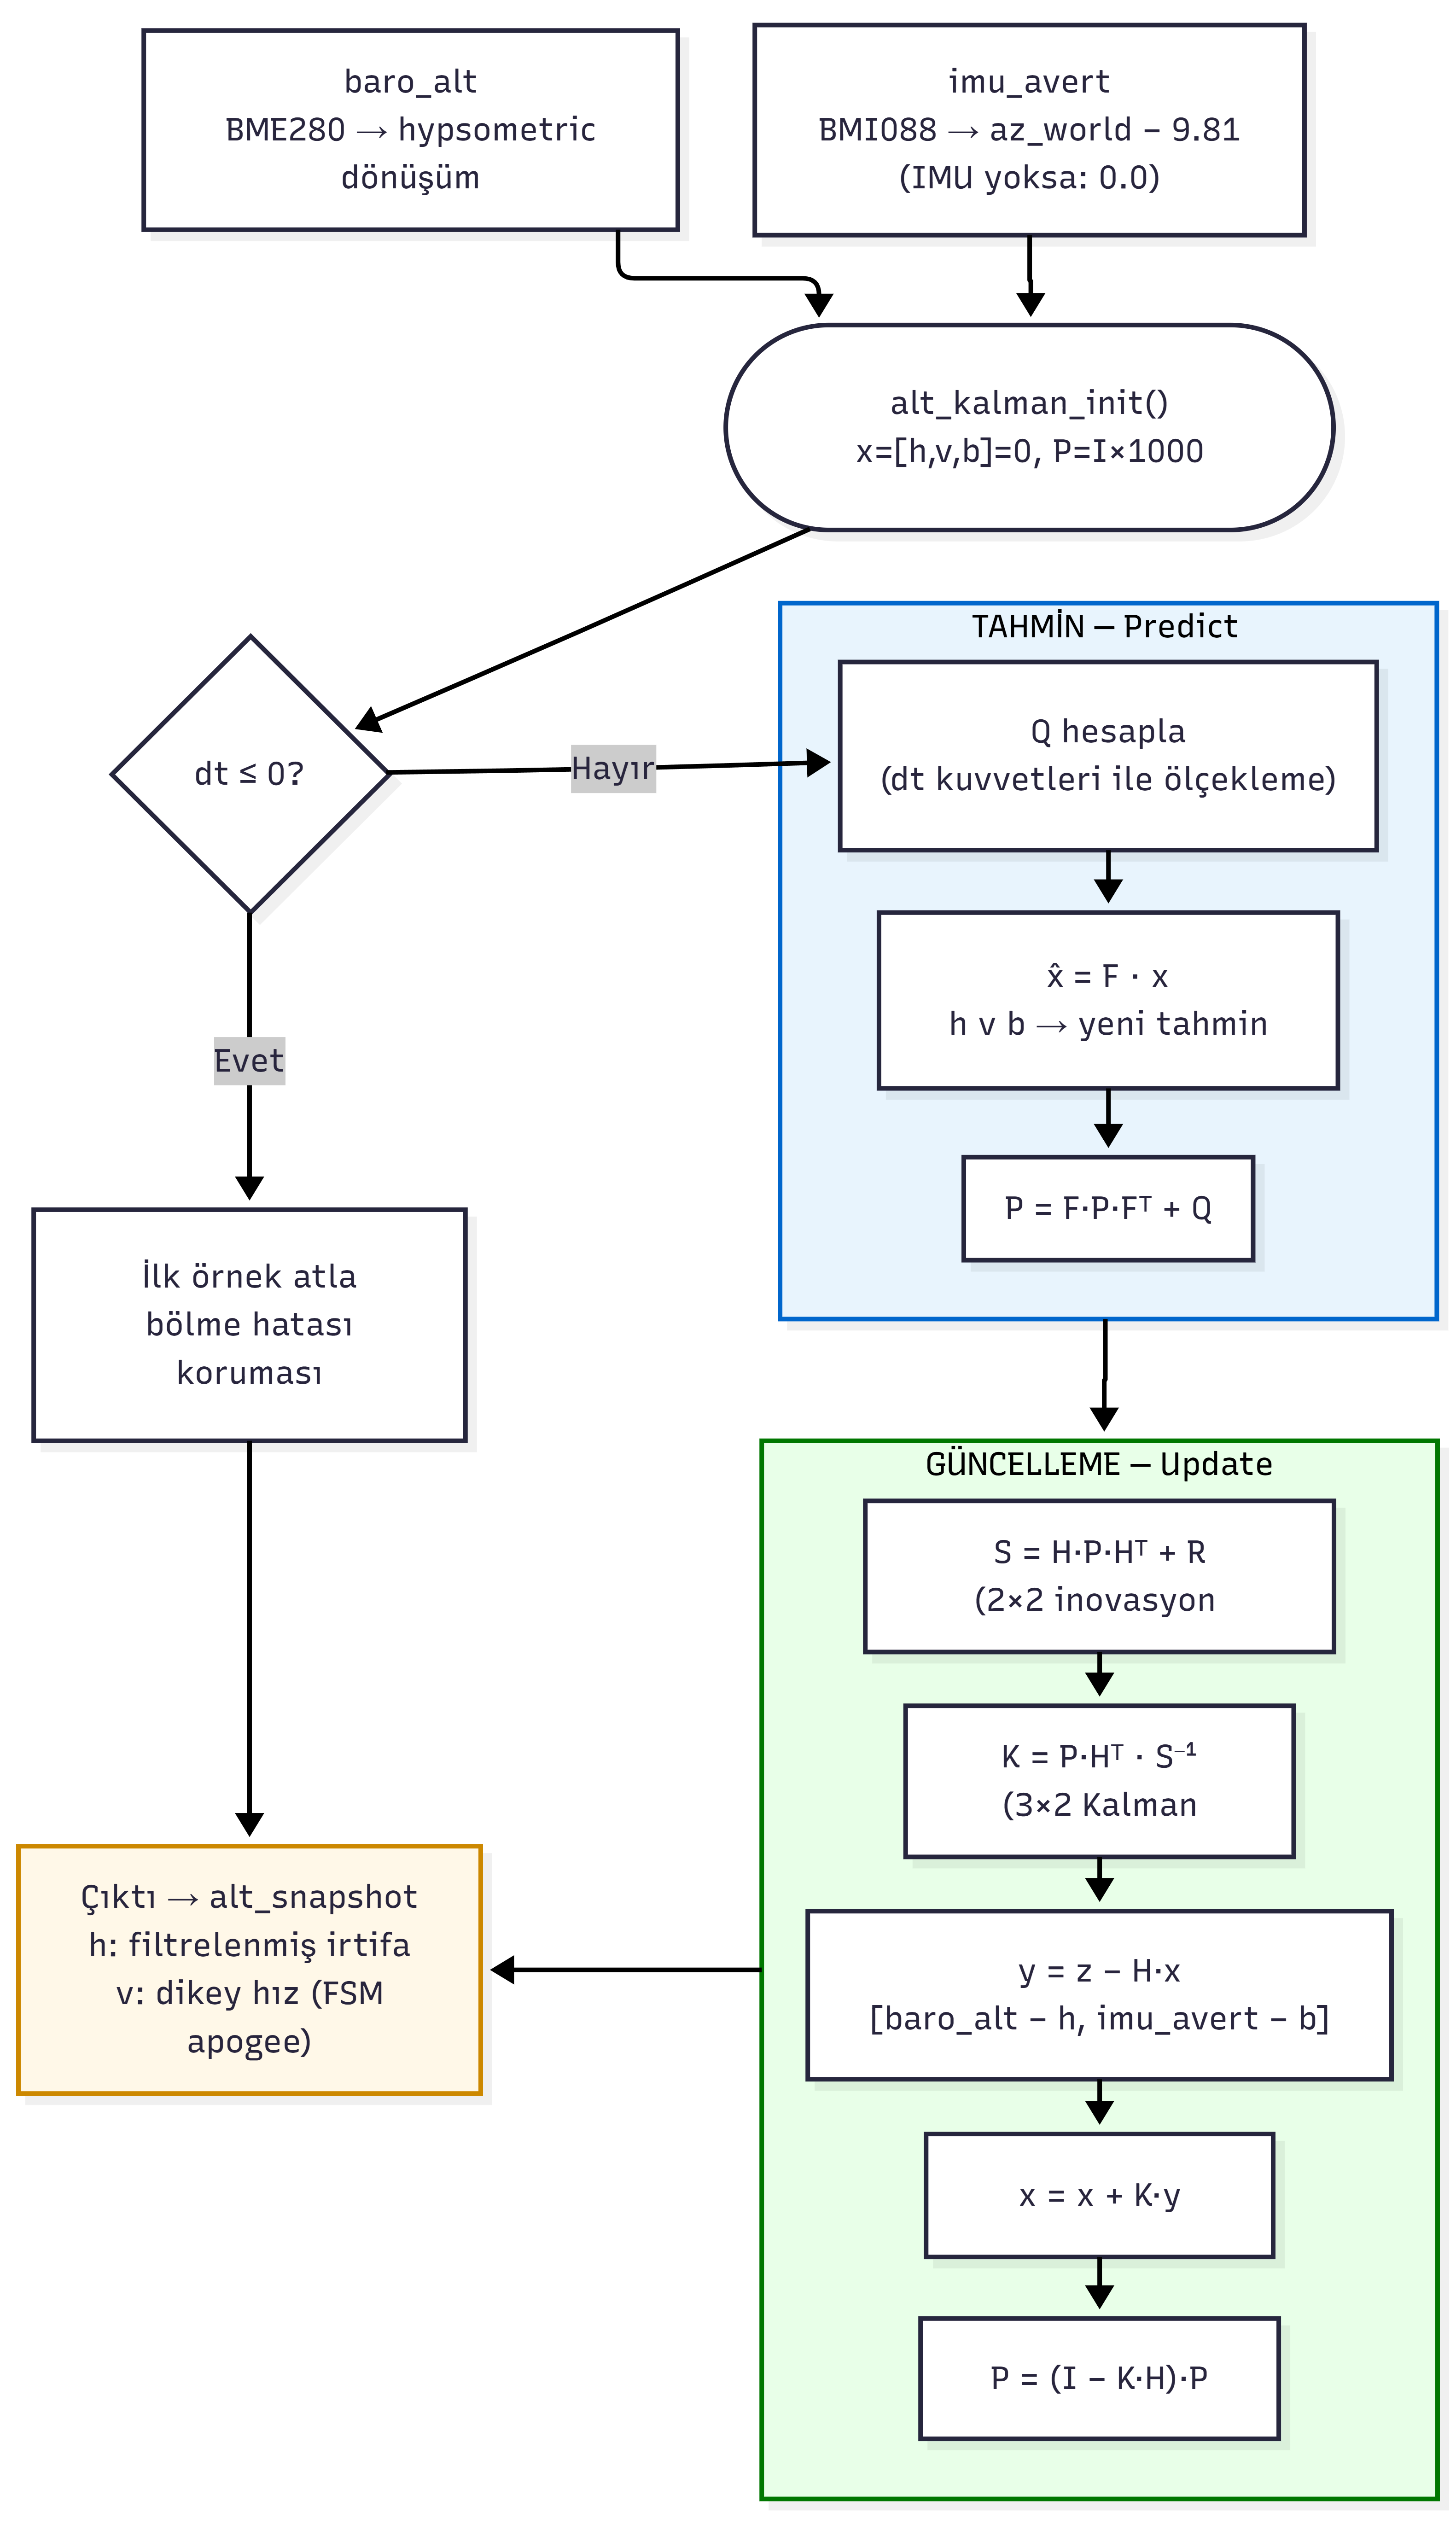
\includegraphics[width=\textwidth]{sekiller/KalmanFiltresi.png}
    \caption{3-Durumlu Baro-IMU Yükseklik Kalman Filtresi Döngüsü}
    \label{fig:kalman_filter}
\end{figure}

Filtrede ayarlanan ($r\_alt = 5.0$, bari gürültüsü) ve ($r\_acc = 10.0$ ivme gürültüsü) gibi varyanslar, filtrenin hangi sensöre daha çok güveneceği ayarını (tuning mantığını) temsil etmektedir. İlk kalkış adımında bölü sıfır hatasının yaşanmaması için \verb|dt <= 0.0f| koruması koda eklenerek kazanç ($K$) oluşturulmuş, son adımda durum matrisleri irtifa ve ivme kullanılarak matris-çarpım tersi ile ($2 \times 2$) güncellenmiştir.

\subsection{Uçuş Durum Makinesi (7 Faz FSM)}
\label{ucus_durum_makinesi}

Model roketin fırlatılışından kurtarma mekanizmalarının ayrılmasına kadarki süreç karmaşık bir Durum Makinesi (Finite State Machine) modülünde ele alınır. 

\begin{itemize}
    \item \textbf{IDLE'dan BOOST'a Geçiş:} Sensörden alınan IMU fırlatma ivmesinin $> 45 m/s^2$ (veya IMU hatasında barometrenin $> 15 m/s$ hız) yakalaması sonucu tetiklenir.
    \item \textbf{BOOST'dan COAST'a Geçiş:} Kalman filtresinin dikey ivmesinin aralıksız 5 örnek ($500 ms$) boyunca $0$'ın altına düşmesi ya da acil durum $8$ sn zaman aşımının oluşmasıyla motordaki yanmanın bittiğine karar verilir. (Burnout).
    \item \textbf{COAST'dan APOGEE'ye Geçiş:} Kalman dikey hızı 0'ın altında kaldığında veya \textit{Tilt (Eğim)} durumu 70 derecenin üzerine çıktığında tespit edilir. Roket apogee (tepe noktasında) olduğunu anladığı anda ilk fırlatma (Drogue) GPIO'su tetiklenir. Çift güvenlik sensörüyle (hem hız, hem açı) tetikleme sağlanır.
    \item \textbf{MAIN DESCENT ve LANDED Geçişi:} İrtifa $300 m$'nin altına indiğinde barometre tetikleyici oluşturur, yere iniş hızı saniyeler (< 2 m/s) ile kesinleştirilip uçuş işlemi sonlandırılır.
\end{itemize}

\begin{figure}[H]
    \centering
    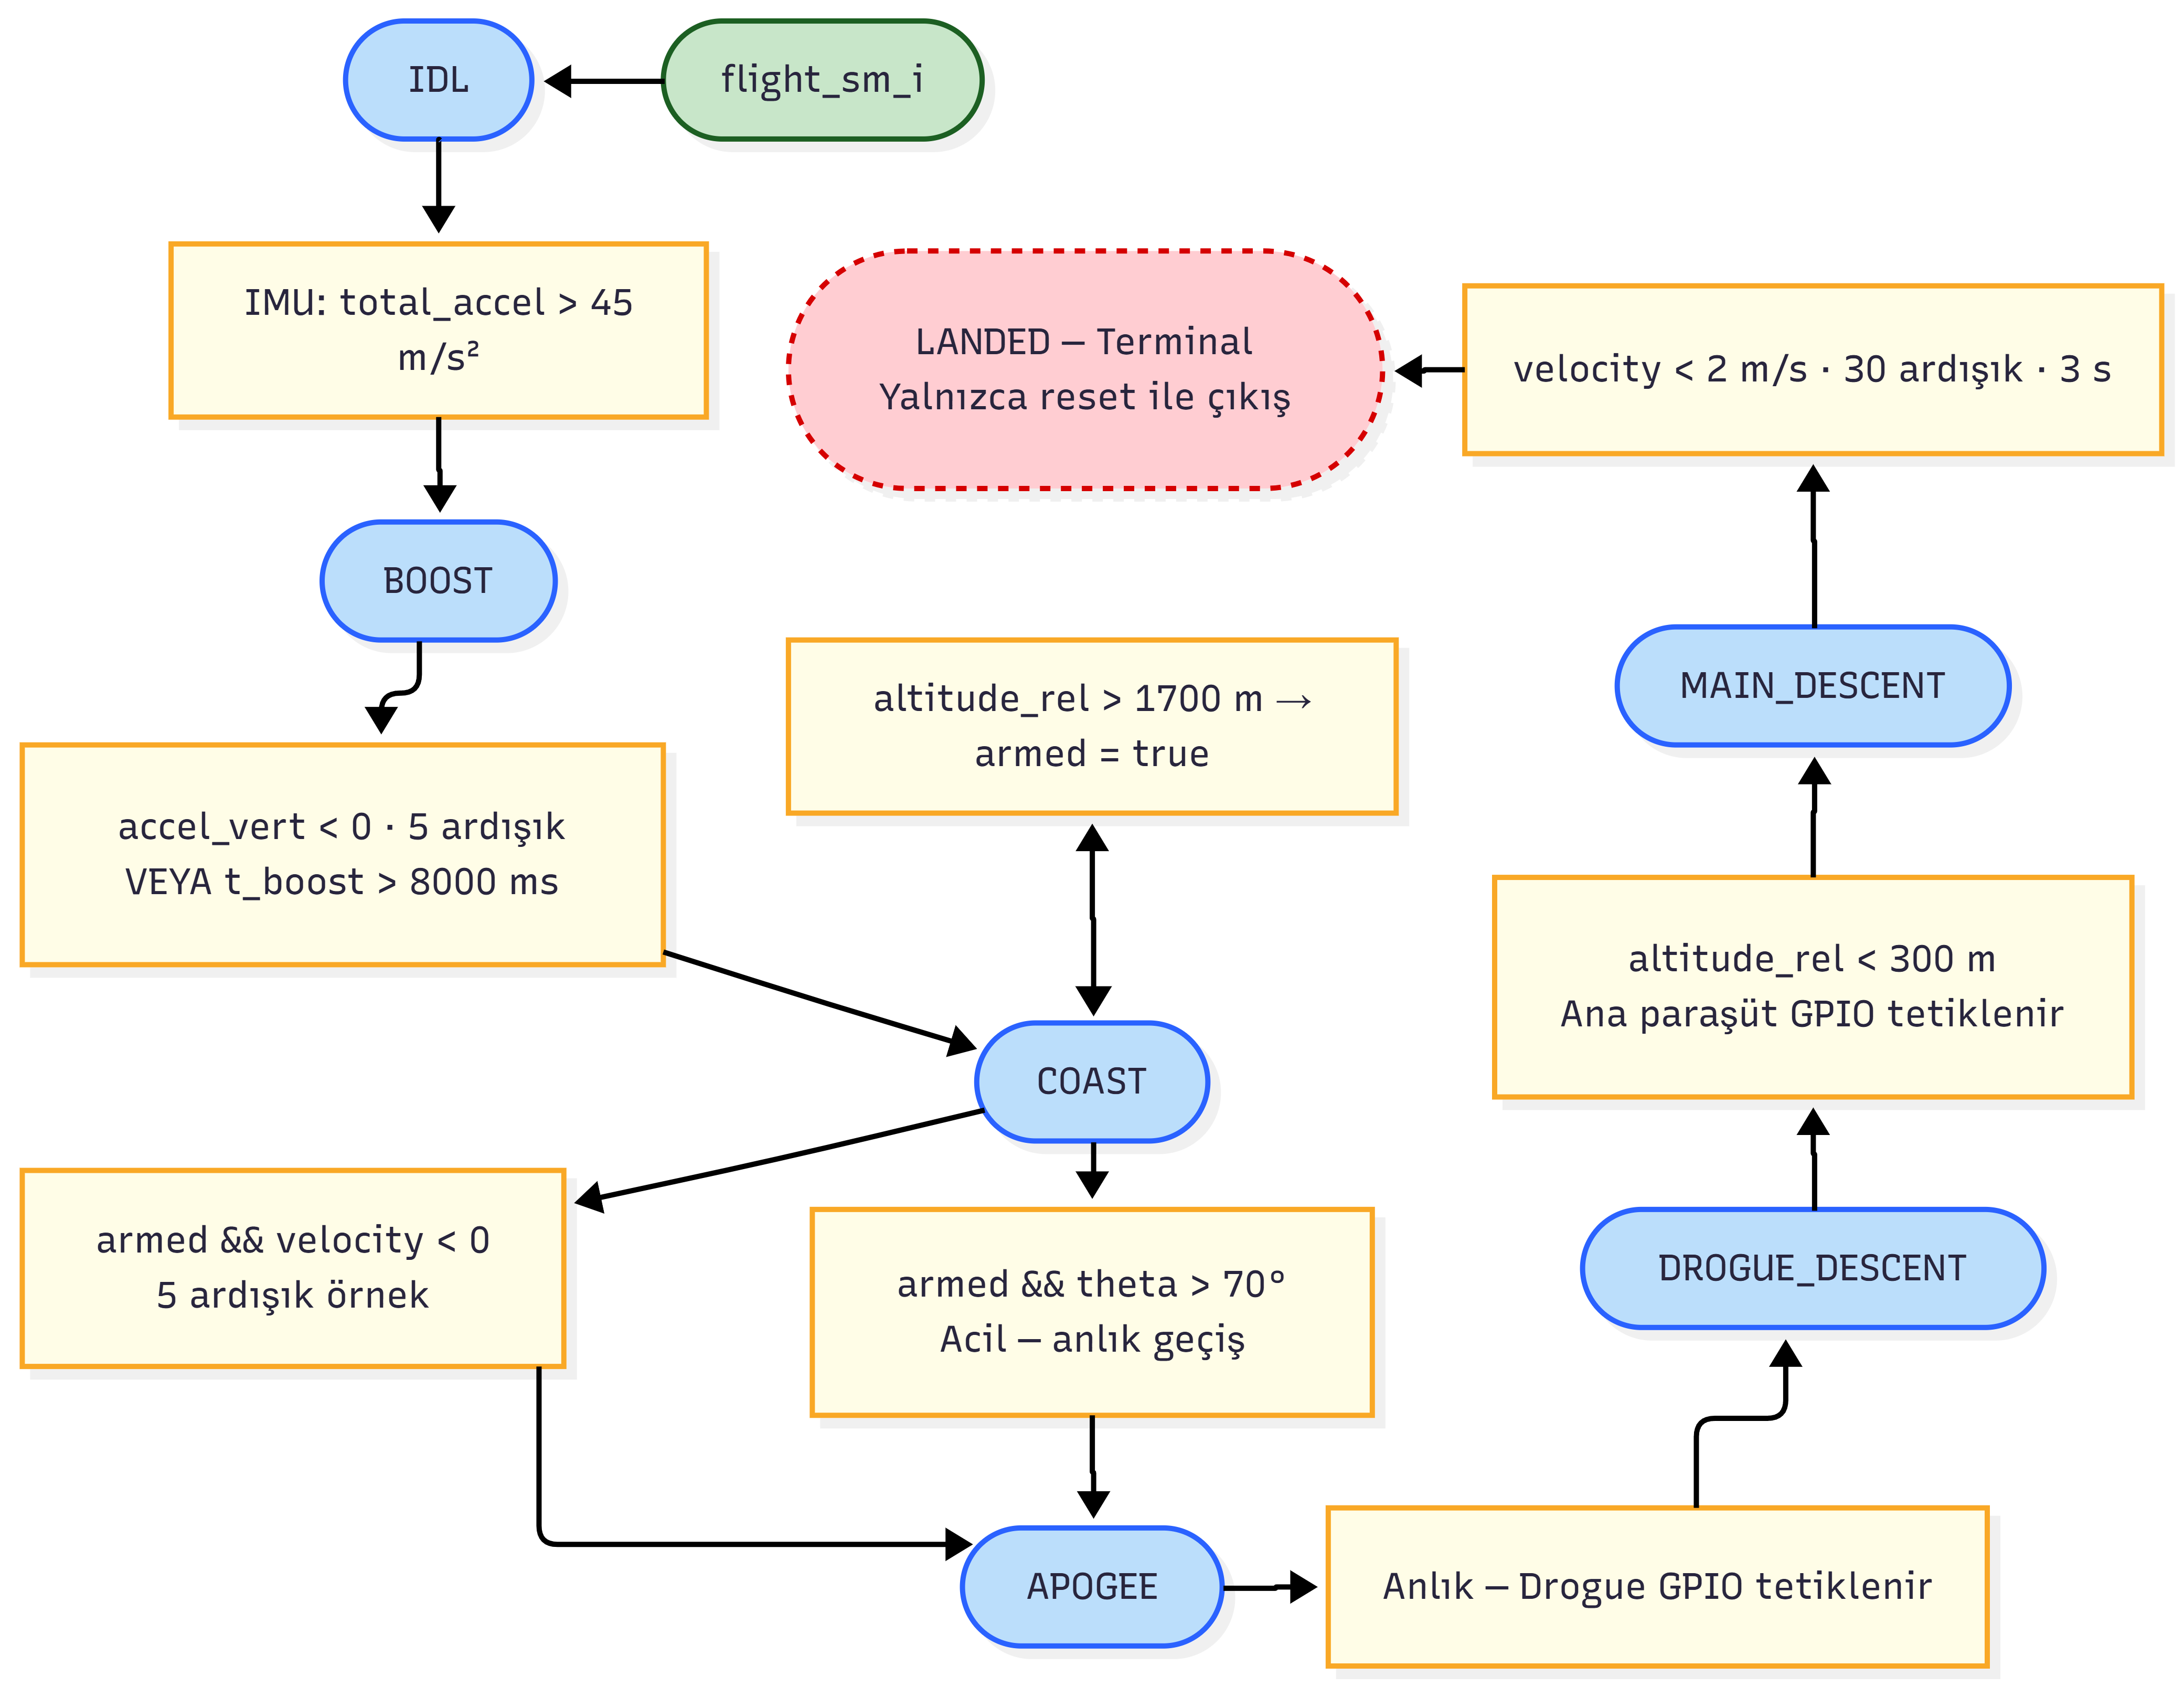
\includegraphics[width=\textwidth]{sekiller/UçuşDurumMakinesi.png}
    \caption{Uçuş Durum Makinesi (FSM) 7-Faz Durum Geçiş Mekanizması}
    \label{fig:ucus_fsm}
\end{figure}

\subsection{Güvenilirlik Mekanizmaları}
\label{guvenilirlik_mekanizmalari}

Dış etmen veya döngü bloklamasından oluşabilecek hayati aviyonik arızalarına karşı aşağıdaki yazılımsal ve donanımsal korumalar entegre edilmiştir.

\subsubsection{IWDG Watchdog ve Yığın Aşım (Stack Overflow) Koruması}
Sistemdeki donanımsal Watchdog $2$ saniyelik zaman aşımına (\textit{timeout}) sahiptir. Barometre görevi (\verb|baro_task|) 100 ms aralıklarla \verb|iwdg_feed()| beslemesi yapar. Eğer görev donarsa, sistem doğrudan kendini sonlandırıp baştan uyanarak sensör veri kurtarmasına gider.
Ayrıca, görevlerin RAM içerisinde kendisine verilenden fazla bir boyutu talep etmesi (Stack Overflow) durumu, sistem başlarken aktive edilen \verb|configCHECK_FOR_STACK_OVERFLOW| ile FreeRTOS kancası (hook) tarafından durdurulup yeniden başlatılmaktadır.

\subsubsection{IMU Başarısızlığında Baro-Only (Kısıtlandırılmış/Degraded) Mod}
Başlangıç durumunda veya kalkıştan sonra \verb|bmi_init| iletişim döngüsünün tam anlamıyla tahrip olması sistemin tamamen kaybolmasına neden teşkil etmez. Sistem böyle bir tabloda; roket fırlatıldı durumunu (BOOST tahmini), sadece hızlanarak kalkan Kalman baro hızı ile sağlar $> 15 m/s$. Ancak tilt-bazlı apogee pasifize edilip, tepe noktasında yedek güvenlik kamerasız çalışır. 

\subsection{Test ve Doğrulama Metodolojisi}
\label{test_ve_dogrulama_metodolojisi}

Model roketin kritik uçuş dinamiklerini simüle edebilmek ve uçuş bilgisayarı algoritmalarını yer istasyonunda test edebilmek amacıyla çeşitli sistem test modülleri (SIT ve SUT) entegre edilmiştir. Bu modüller donanım ile bilgisayar (Python arayüzü) arasındaki köprüyü oluşturmaktadır.

\subsubsection{SIT — Sensör İzleme Testi}
Bu metodoloji, sensör verilerinin doğrudan mikrodenetleyiciden okunarak bir bilgisayar ortamına (Python GUI) yansıtılıp canlı incelenmesini hedefler. Algoritmaların doğru çalışıp çalışmadığını değil; STM32 ve sensörler arasındaki donanımsal sürücü iletişim yollarını (DMA, I2C, USART2 transferleri) doğrulamak amaçlanmıştır. 

Statik ortam testinde IMU çıktılarının (Z ekseni yaklaşık -9.81 $m/s^2$ yerçekimi ivmesi olacak haliyle) doğruluğu, barometrik irtifanın bulunulan konum koşullarıyla uyuşmazlığı hesaplanarak Mahony denklemlerinden roll, pitch, yaw gibi veriler de 3 boyutlu roket dönüşüm modelinde görselleştirilir.

\begin{figure}[H]
    \centering
    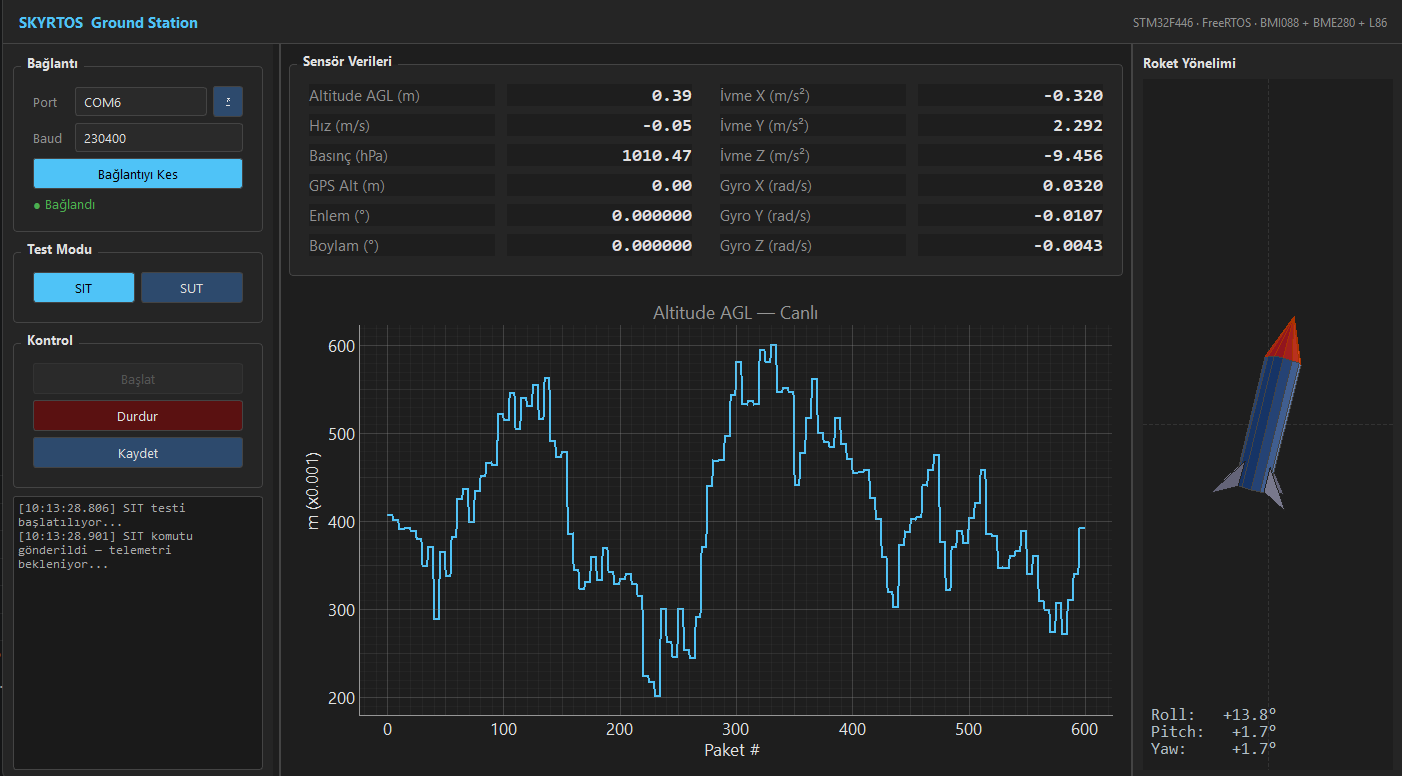
\includegraphics[width=\textwidth]{sekiller/SIT_testi_arayüz.png}
    \caption{Python GUI Canlı Sensör İzleme ve Yönelim 3D Görselleştirmesi (SIT)}
    \label{fig:sit_test}
\end{figure}

\begin{table}[H]
    \centering
    \caption{SIT Test Senaryoları ve Beklenen Yanıtlar}
    \label{tab:sit_senaryolar}
    \begin{tabular}{|p{4cm}|p{6cm}|p{5cm}|}
    \hline
    \textbf{Test Olayı} & \textbf{Beklenen Tepki} & \textbf{Test Durumu} \\ \hline
    Masaüstü Statik Test & Z İvmesi: $-9.81 m/s^2$, X ve Y: $\sim 0$ & Kalibrasyon ve referans uyumu sağlandı. \\ \hline
    Euler ve Quaternion İzleme & XYZ Ekseninde 3 Boyutlu Dönüşler & Gimbal Lock açmazı engellendi, yansıması başarılı. \\ \hline
    Baro Referans Doğrulaması & 0 Metre Rölatif (Göreli) İrtifa Set Edilmeli & Çevresel stabilite, ofset sıfırlandı. \\ \hline
    \end{tabular}
\end{table}

\subsubsection{SUT — Sentetik Uçuş Testi (Processor-in-the-Loop)}
SUT metodolojisinde ("Processor-in-the-Loop"), algoritma tepkilerini ve 7-faz FSM kararlarını test etmek maksadıyla RocketPy \cite{rocketpy} açık kaynak simülatöründen faydalanılmıştır. Bu test modunda, PC simüle edilmiş ivme ve irtifa okumalarını UART üzerinden peyderpey STM32 uçuş bilgisayarına yollar. 

Bu süreçte STM32'de yeralan \verb|imu_task|, \verb|baro_task|, \verb|telemetry_task| ve \verb|gnss_task| modülleri \verb|MODE_SUT| kontrolüne takılarak \verb|portMAX_DELAY| ile uyutulur; CPU simüle edilmiş \verb|sut_task| tarafından harcanır. Sistem, PC den aldığı verileri Mahony ve Kalman filtrelerinden geçirir ve Python platformuna Cevap Paketi (SUT\_RESPONSE) olarak aynen iletir.

SUT Haberleşme yapısında kullanılan temel cevap paketi formatı alt kısımda tablolanmıştır (STM32 den PC'ye):
\begin{table}[H]
    \centering
    \caption{SUT Response UART Paketi İçeriği (Toplam 26 Bayt)}
    \label{tab:sut_response}
    \begin{tabular}{|l|l|l|l|}
    \hline
    \textbf{Offset} & \textbf{Bayt / Veri Tipi} & \textbf{Paket İçeriği} \\ \hline
    0 & 1 (uint8\_t) & Başlangıç Header (0xAE) \\ \hline
    1 - 4 & 4 (float) & Simülasyon Zamanı (sim\_time) \\ \hline
    5 - 8 & 4 (float) & Filtrelenmiş İrtifa Verisi \\ \hline
    9 - 20 & 12 (3 x float) & Roll, Pitch ve Yaw Deg Açıları \\ \hline
    21 - 22 & 2 (uint16\_t) & FSM Durumu (HIGH/LOW Byte) \\ \hline
    23 & 1 (uint8\_t) & Sağlama Toplamı (Checksum) \\ \hline
    24 - 25 & 2 & Bitiş (0x0D, 0x0A - CR LF) \\ \hline
    \end{tabular}
\end{table}

\begin{figure}[H]
    \centering
    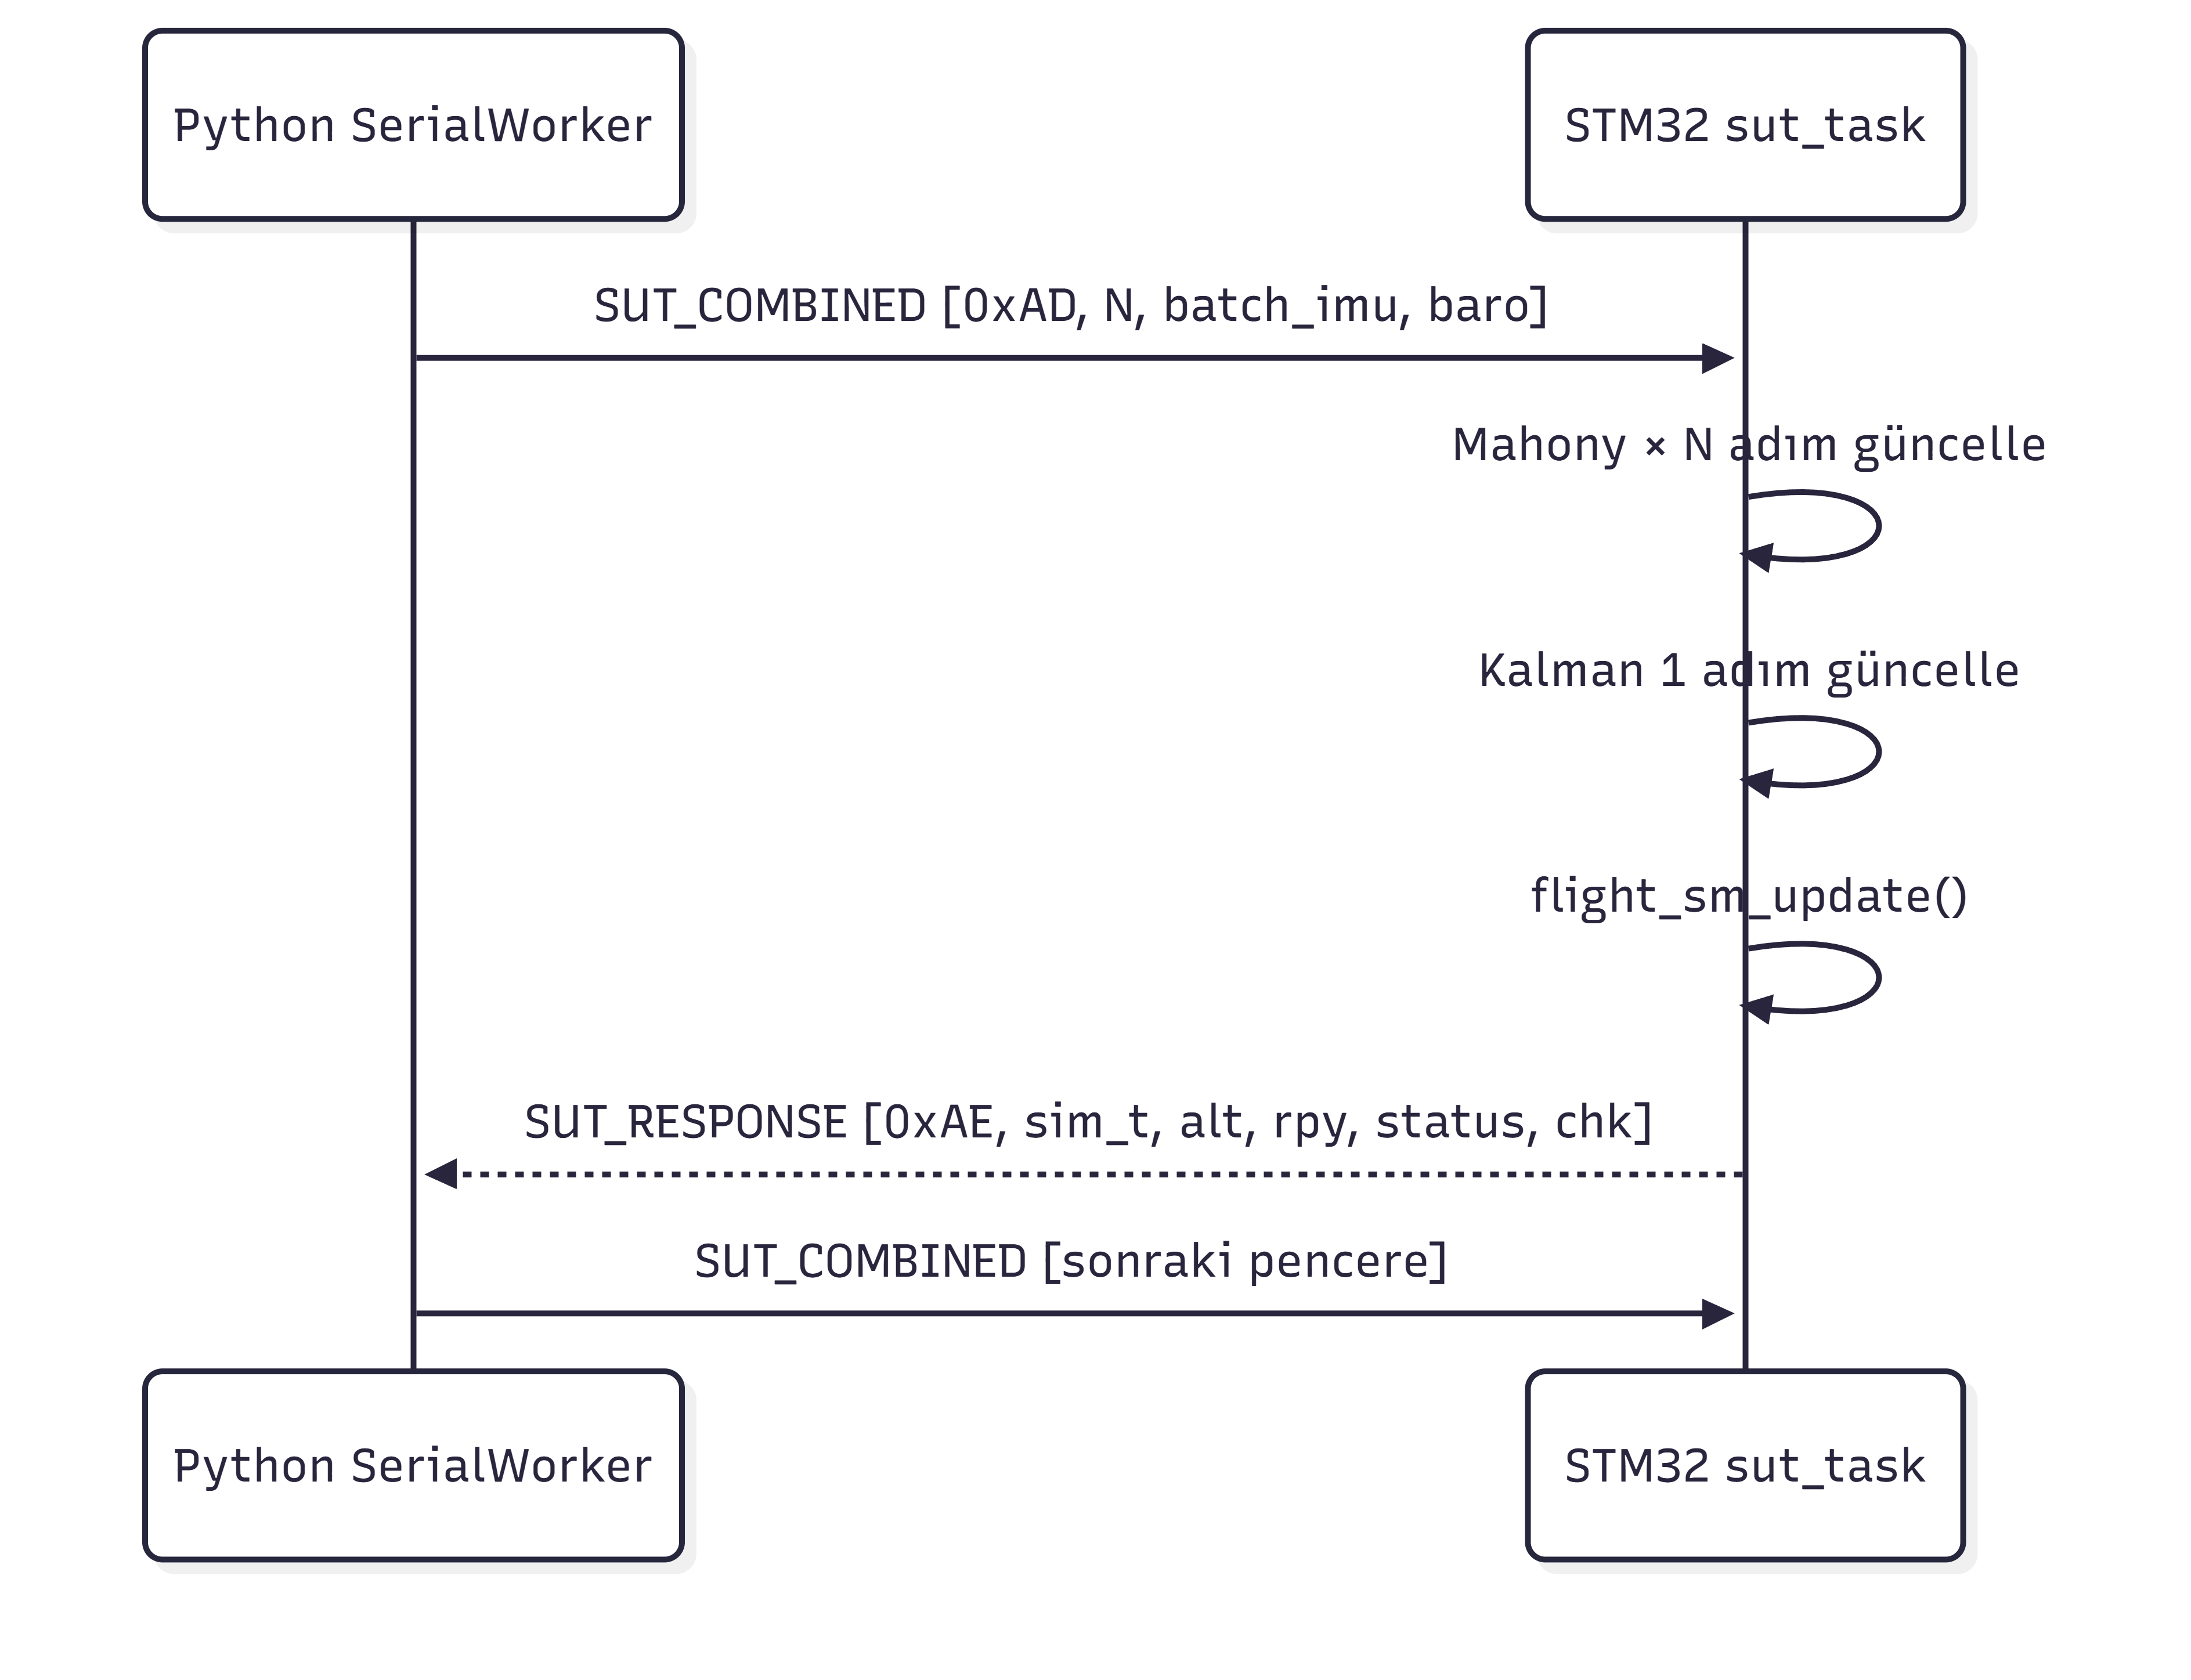
\includegraphics[width=0.8\textwidth]{sekiller/SUT_SistemMimarisi.png}
    \caption{Processor-in-the-Loop Veri Aktarım Akışı (SUT)}
    \label{fig:sut_mimarisi}
\end{figure}

Aşağıdaki pseudo-code (sözde kod), STM32 \verb|sut_task| dairesel veri analiz mimarisini yansıtmaktadır:
\begin{lstlisting}[language=C, caption={SUT İşleyişi Pseudo-Code Özeti}]
// cmd_task ile iletilen bildirimler
if (sut_queue_receive(&pkt)) {
    for (int i = 0; i < pkt.imu_count; i++) {
        // Gyro-only (Mahony Batch hesaplamalari)
        mahony_update(&mah, pkt.imu[i].gx ... dt); 
    }
    float filtered = alt_kalman_update(&kf, alt_rel, 0.0f, dt_baro);
    flight_sm_update(&alt_snap, &imu_snap);
    sut_send_response(..., filtered, roll, pitch, yaw, flight_status);
}
\end{lstlisting}

\subsubsection{RocketPy Simülasyon Verisi ve Test Altyapısı}
Simülatöre girdi olarak \textbf{RocketPy} ortamı kullanılmış ve aviyonik karta sentetik olarak yollanacak sanal atmosferik ile statik veriş akışı CSV tablolarına kaydedilmiştir. Sisteme entegre edilen Python parametreleri gereksinimlerin testine olanak tanır:

\begin{figure}[H]
    \centering
    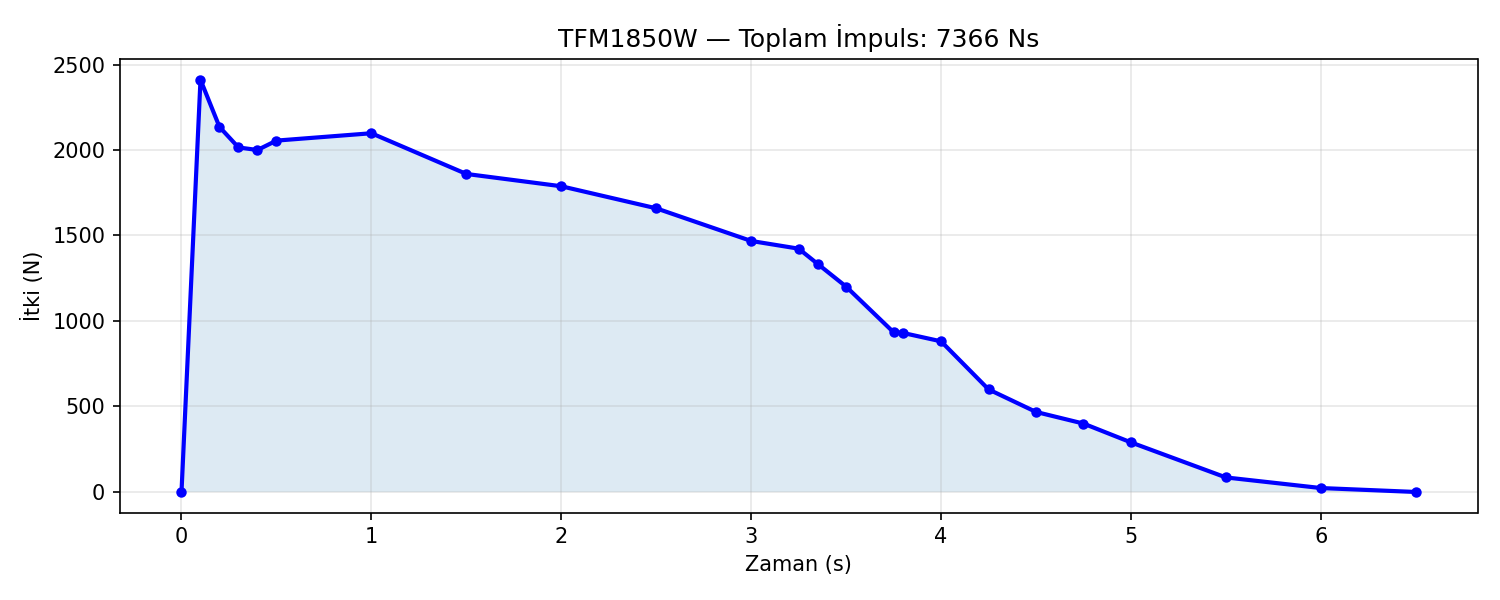
\includegraphics[width=0.8\textwidth]{sekiller/motor_thrust.png}
    \caption{RocketPy Simülasyonunda Kullanılan Motor İtme Kuvveti (Thrust) Eğrisi}
    \label{fig:motor_thrust}
\end{figure}

\begin{lstlisting}[language=Python, caption={RocketPy Motor, Roket Boyutları ve Atmosfer Ortamı Tanımlamaları}]
from rocketpy import SolidMotor, Rocket, Environment

motor = SolidMotor(
    thrust_source="data/TFM1850W.eng",  # Itme egrisi
    dry_mass=6.693,                     # Kuru kutle (kg)
    burn_time=6.5,                      # Yanma suresi (s)
    # diger degiskenler ...
)

rocket = Rocket(
    radius=0.056,                       # Govde yaricapi (56 mm)
    mass=15.166,                        # Motorsuz kuru kutle
    power_off_drag=0.45,                
    power_on_drag=0.45,
    center_of_mass_without_motor=1.13,  # CG, kuyruktan (m)
)
rocket.add_motor(motor, position=0.0)

env = Environment(
    latitude=39.90, longitude=32.80, elevation=900.0  # Ankara referansi
)
env.set_atmospheric_model(type="standard_atmosphere")
\end{lstlisting}

Simülasyon sonucunda elde edilen teorik irtifa ve ivme grafikleri sensörlerin SUT modu üzerinden test edilmesi için temel referans modelleri olarak CSV dosyalarına kaydedilmektedir.

\begin{figure}[H]
    \centering
    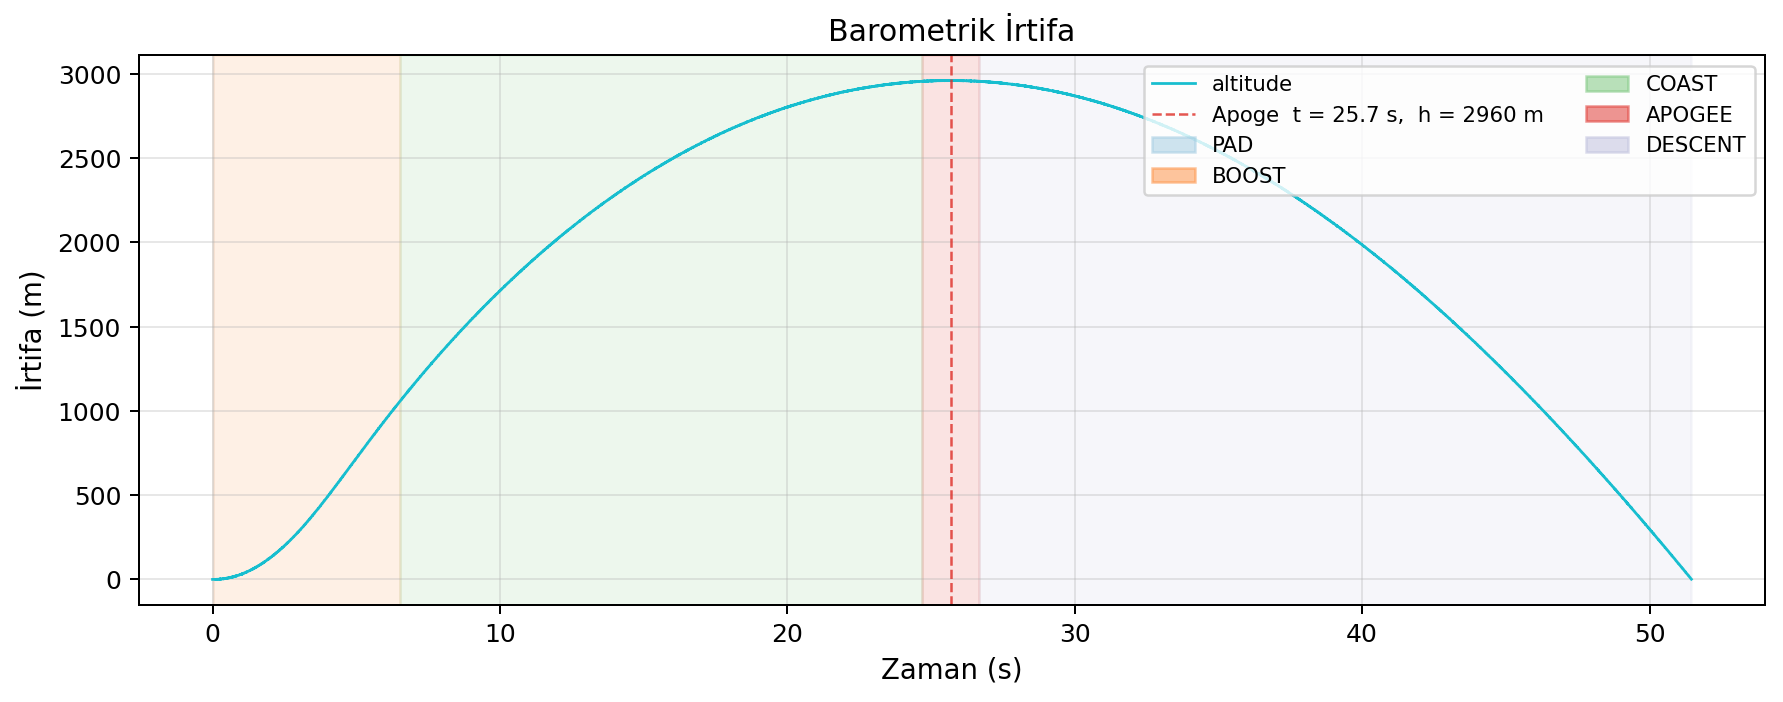
\includegraphics[width=0.8\textwidth]{sekiller/fig_altitude.png}
    \caption{RocketPy Simülasyonu Teorik İrtifa-Zaman Grafiği}
    \label{fig:rocketpy_altitude}
\end{figure}

\begin{figure}[H]
    \centering
    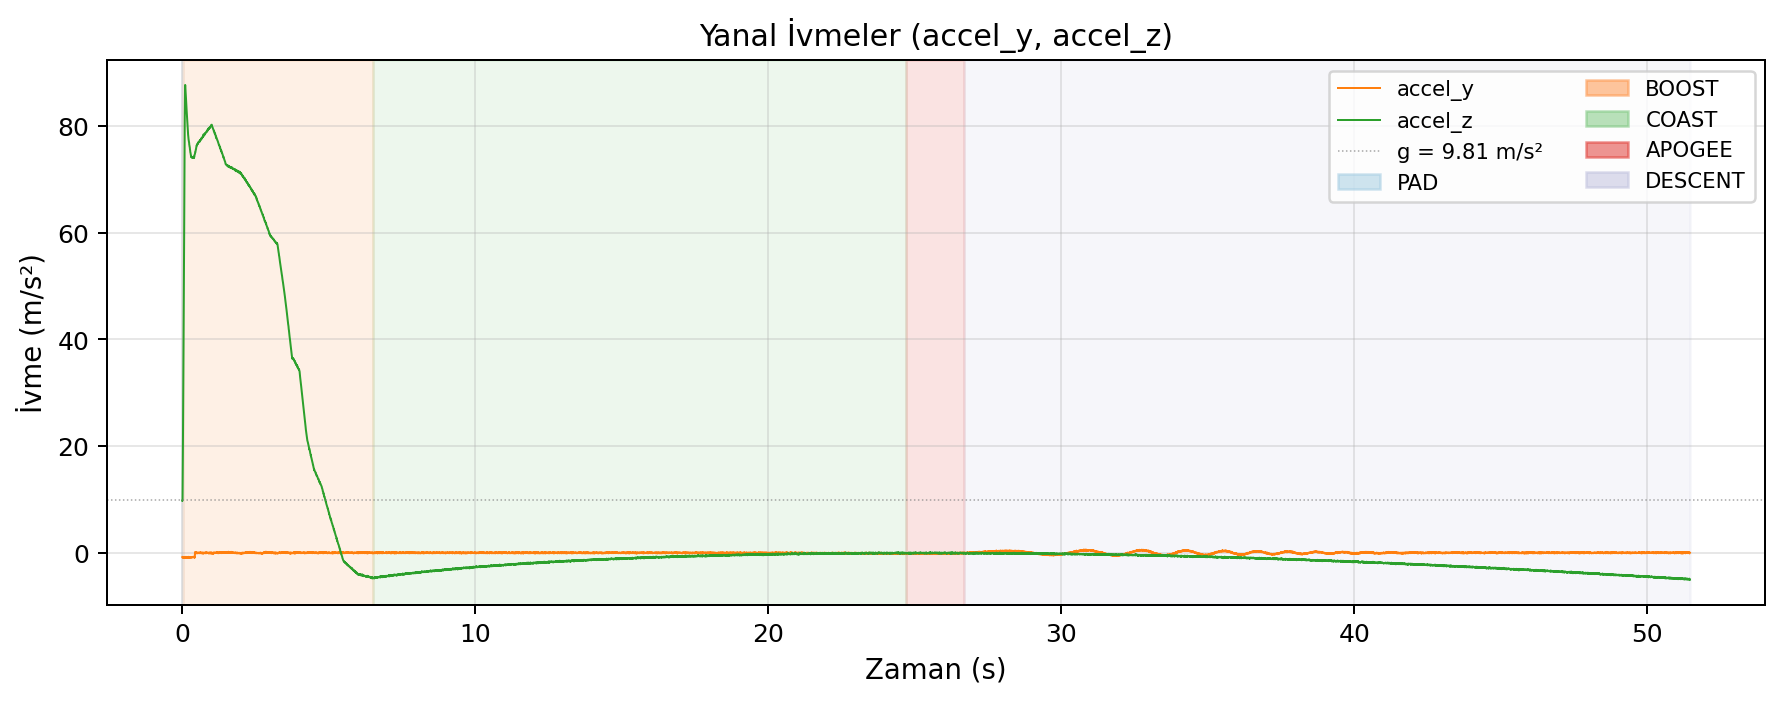
\includegraphics[width=0.8\textwidth]{sekiller/fig_accel_yz.png}
    \caption{RocketPy Simülasyonu Teorik İvme (Y-Z Ekseni) Grafiği}
    \label{fig:rocketpy_accel}
\end{figure}

Algoritmalar bu sistem üzerinde koşturulduktan sonra STM32 tarafından "PyQtGraph" ekranına (Hız, zaman, İvme vb.) durum çizgisi basılarak uçuş evresi analiz edilmektedir.

\clearpage
\section{BÖLÜM IV}
\label{bolum4}

\subsection{Bulgular}

Tezinizin bulgularını ortaya koyduğunuz bölümdür. Yani tezinizin asıl bölümü burasıdır denilebilir. Bulgular bölümünde, araştırma sorularınızın cevapları yer alır. Ancak yorumlara girilmez. Çünkü bunlar sonraki bölümde yazılacaktır. 


\clearpage
\section{BÖLÜM V}
\label{bolum5}

\subsection{Tartışma ve Sonuçlar}
Bu bölüm bulgular bölümünde ortaya koyduğunuz sonuçların derli toplu olarak ifade edildiği, bunlara dayalı olarak çıkarım ve yorumlarınızın verildiği bölümdür. Bu yönüyle, bulgular gibi tezinizin en önemli bölümüdür. Bu bölümde sizden bu çalışma sonucunda ne(ler) bulduğunuzu ortaya koymanız istenir. 

Ayrıca, bu sonuçların literatür taramasında bulduğunuz hangi sonuçlara benzediği veya benzemediğini ifade etmeniz beklenir. Buna tartışma adı verilir. Son olarak da bu bölümde çalışmanız ile ilgili olarak önerilerinizi sunmanız gerekir. Sonuç bölümü; tartışma ve sonuç, sonuç ve öneriler gibi farklı başlıklar alabilir. Ayrıca, bölüm içerisinde 1-sonuç ve 2-öneriler gibi alt başlıklar koymanız istenebilir. 

\clearpage
%\clearpage
\section{Gantt Şeması}
\label{gantt}

Çalışma planına ait iş paketleri (tanımları) aşağıdaki gibi tanımlanmalı ve Gantt şeması  kullanılarak gösterilmelidir. En az 4 adet iş paketi tanımlanmalıdır. İş paketlerinde proje grubu elemanlarının hangi görevi yapacakları belirtilmelidir.
\begin{enumerate}
\item İP.1. İş Paketi Adı: Açıklaması
\item İP.2. İş Paketi Adı: Açıklaması
\end{enumerate}


\begin{table*}[!h]
\centering
    \renewcommand{\arraystretch}{1.5}
        \begin{tabular}{| c | c | c | c | c | c | c | c | c | }
              \hline
              \multirow{2}{*}{\parbox{0in}\textbf{{Aylar}}}
              & & & & & & & & \\ \cline{2-9}
              & 11 & 12 & 1 & 2 & 3 & 4 & 5 & 6 \\ \hline

              \multirow{5}{*}{\parbox{0in}\textbf{{İş Tanımı}}}
              						& \multicolumn{3}{c}{\textbf{İP.1}} & & & & & \\ \cline{2-9}
              						& & \multicolumn{4}{|c|}{\textbf{İP.1}} & & & \\ \cline{2-9}
              						& & & & & & & & \\ \cline{2-9}
              						& & & & & & & & \\ \cline{2-9} \hline
    \end{tabular}%}
    \newline
        \caption{Gantt Şeması}
        \label{table:gantt}
    \renewcommand{\arraystretch}{1} 
\end{table*}

\clearpage

\bibliographystyle{IEEEtran} 
\bibliography{referanslar}	 

%\appendix
%\clearpage
\section{Ek 1}
\label{ek}

Var ise kodlarınızı uygun formatta buraya ekleyiniz.

\begin{lstlisting}
 /*  * Usage of printf() function.  */  

#include <stdio>  
main () {
	printf();
	}
\end{lstlisting}

\end{document}
